\documentclass[aspectratio=169]{beamer}

\usetheme{Madrid}
\usecolortheme{default}
\setbeamertemplate{navigation symbols}{}
\setbeamertemplate{footline}[frame number]

\usepackage[utf8]{inputenc}
\usepackage[T1]{fontenc}
\usepackage{amsmath, amssymb}
\usepackage{booktabs}
\usepackage{multirow}
\usepackage{tikz}
\usepackage{pgfplots}
\pgfplotsset{compat=1.18}
\usetikzlibrary{arrows.meta, positioning, fit, backgrounds, matrix}
\usepackage{graphicx}
\graphicspath{{presentation_assets/}}

\definecolor{iiitblue}{RGB}{0,77,128}
\definecolor{iiitgreen}{RGB}{36,110,92}
\definecolor{iiitorange}{RGB}{200,110,35}
\setbeamercolor{structure}{fg=iiitblue}
\setbeamercolor{title}{fg=iiitblue}
\setbeamercolor{frametitle}{fg=iiitblue}

\title{Graph-Aware Stance Detection for Syncialo}
\subtitle{Motivation, Experiments, Theory, and Interpretation}
\author{BTP Research Presentation}
\institute{Indian Institute of Information Technology Kottayam}
\date{\today}

\begin{document}

\begin{frame}{Title}
  \titlepage
\end{frame}

\begin{frame}{Presentation Roadmap}
  \tableofcontents
\end{frame}

\section{Motivation}

\begin{frame}{Motivation and Research Direction}
The original system already had:
\begin{itemize}
  \item Strong pairwise stance signals from transformer models
  \item Graph construction and graph algorithms for debate analysis
\end{itemize}

The core bottleneck was that the graph analysis was only as good as the stance predictions.

Our central research question is:
\begin{block}{Research Question}
Can we improve stance detection by incorporating debate-local graph structure rather than classifying each claim pair in isolation?
\end{block}
\end{frame}

\begin{frame}{Why the Previous System Was Bottlenecked}
The older presentation already identified the central limitation:
\begin{itemize}
  \item The graph modelling and graph algorithms were in place
  \item The overall system still struggled on complex debates
  \item The main bottleneck was the stance prediction module
\end{itemize}

This motivates a progression of experiments:
\begin{enumerate}
  \item Direct NLI baseline
  \item Direct stance baseline
  \item Fused DeBERTa + stance logistic regression baseline
  \item Graph-aware model with debate-local semantic structure
\end{enumerate}
\end{frame}

\begin{frame}{Legacy Pipeline Context}
  \begin{columns}[T]
    \begin{column}{0.54\textwidth}
      The previous framework treated the problem as a modular pipeline:
      \begin{itemize}
        \item Claim extraction
        \item Stance detection
        \item Graph construction
        \item Graph analysis
        \item Contradiction and cycle reasoning
      \end{itemize}

      The new work preserves this structure but focuses on improving the stance component so that downstream graph reasoning becomes more reliable.
    \end{column}
    \begin{column}{0.42\textwidth}
      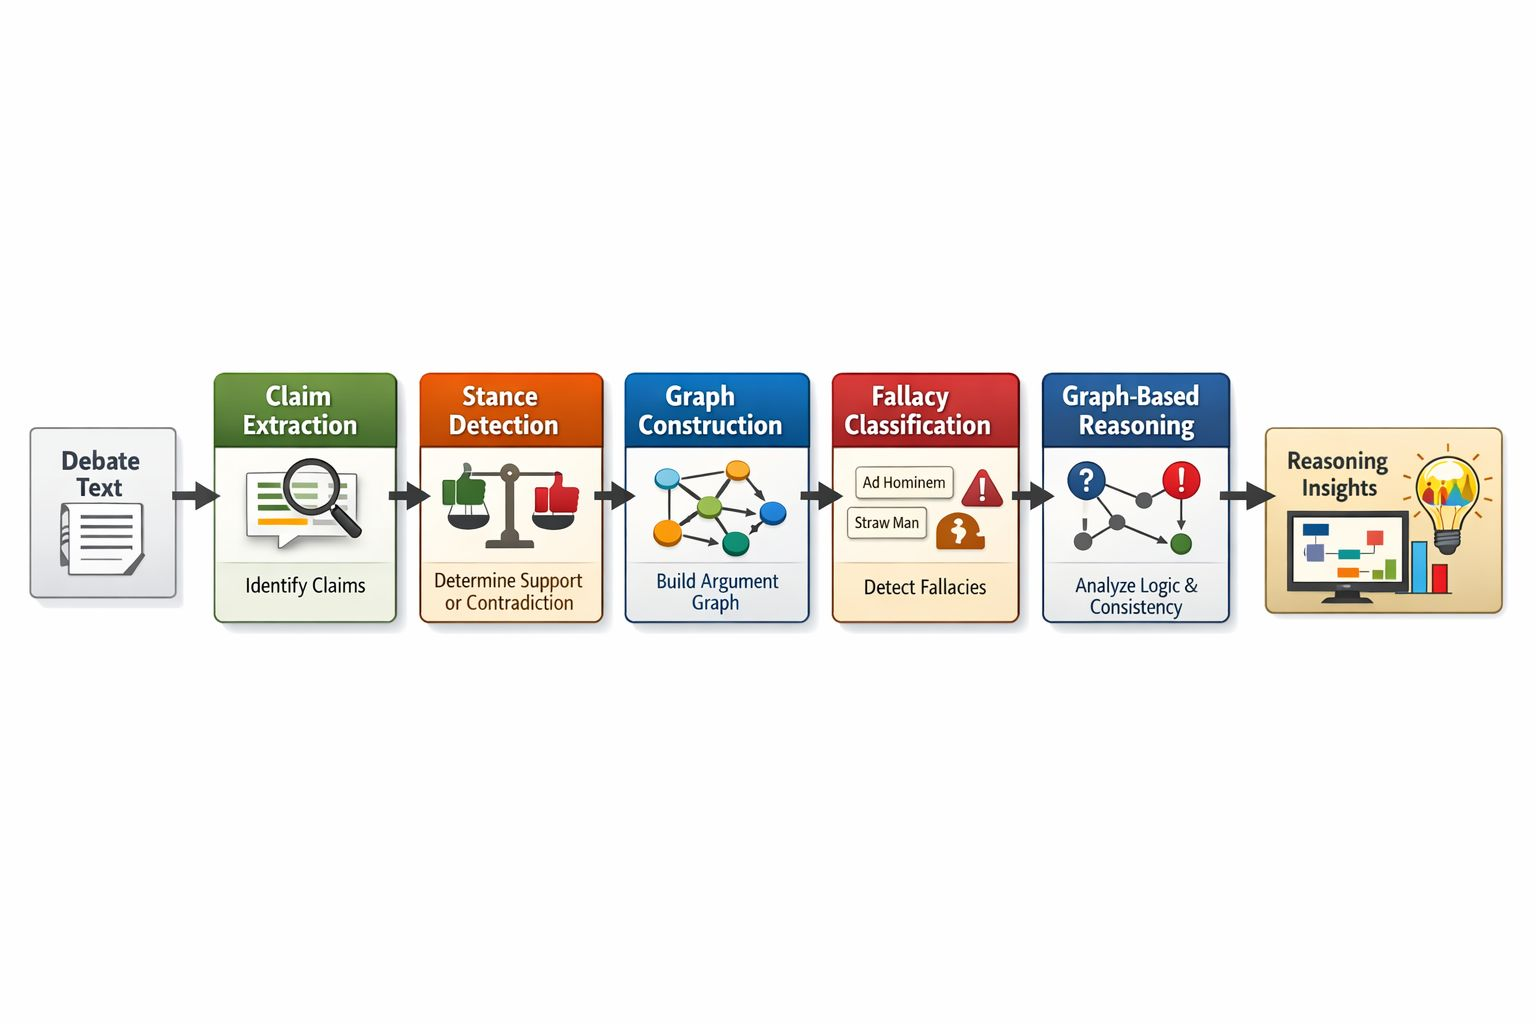
\includegraphics[width=\linewidth]{1.jpg}
    \end{column}
  \end{columns}
\end{frame}

\section{Problem and Data}

\begin{frame}{Problem Formulation}
Each candidate edge is a directed relation:
\[
e = (u,v,y)
\]
where:
\begin{itemize}
  \item \(u\): source claim
  \item \(v\): target claim
  \item \(y \in \{\texttt{support}, \texttt{attack}, \texttt{neutral}\}\)
\end{itemize}

The textual convention used throughout the experiments is:
\begin{itemize}
  \item Premise \(=\) target claim text
  \item Hypothesis \(=\) source claim text
\end{itemize}
\end{frame}

\begin{frame}{Dataset and Benchmark Setup}
  \begin{columns}[T]
    \begin{column}{0.55\textwidth}
      Dataset used for benchmarking:
      \begin{itemize}
        \item SyncIALO, a synthetic Kialo-style debate graph dataset
        \item Corpus: \texttt{synthetic\_corpus-001}
        \item Split used in the saved benchmark: \texttt{eval}
      \end{itemize}

      Saved benchmark configuration:
      \begin{itemize}
        \item Debates used: \(8\)
        \item Train debates: \(6\)
        \item Test debates: \(2\)
        \item Training examples: \(7224\)
        \item Test examples: \(2664\)
      \end{itemize}
    \end{column}
    \begin{column}{0.4\textwidth}
      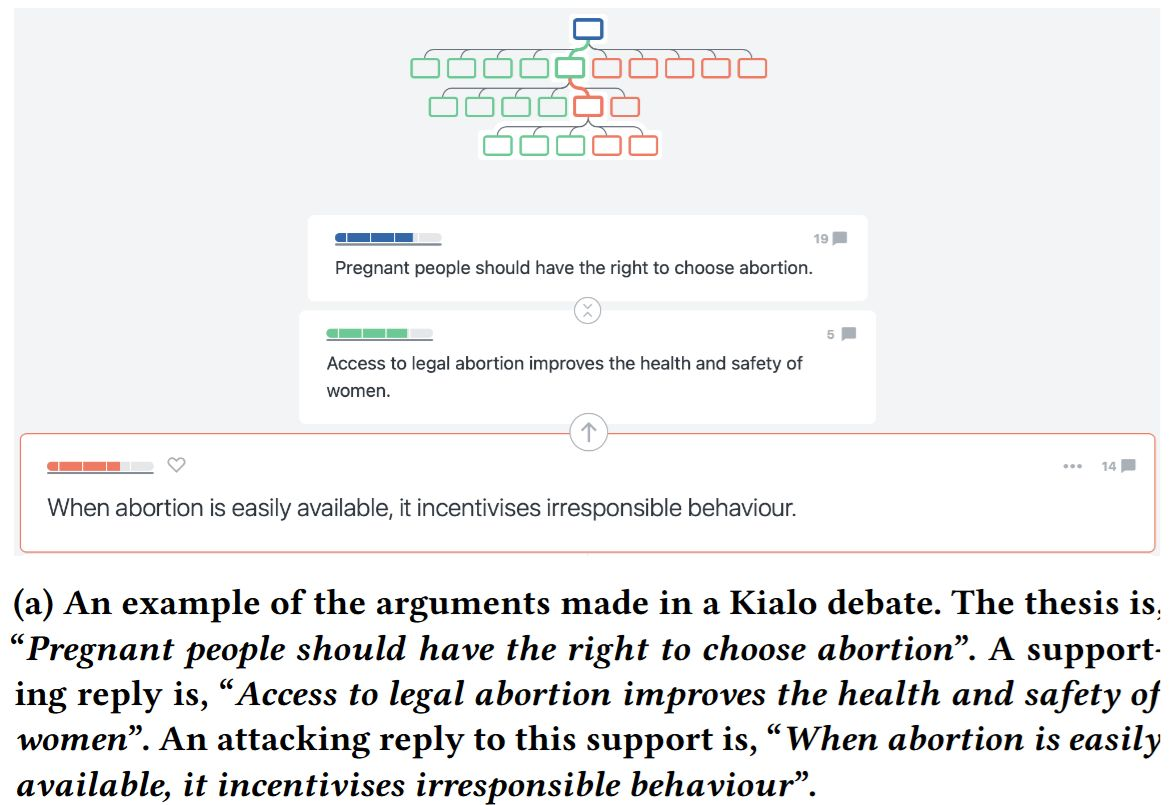
\includegraphics[width=\linewidth]{8.jpg}
    \end{column}
  \end{columns}
\end{frame}

\begin{frame}{Class Distribution}
\centering
\begin{tabular}{lrrrr}
\toprule
Split & Support & Attack & Neutral & Total \\
\midrule
Train & 1806 & 1806 & 3612 & 7224 \\
Test & 666 & 666 & 1332 & 2664 \\
Overall & 2472 & 2472 & 4944 & 9888 \\
\bottomrule
\end{tabular}

\vspace{0.6cm}
Observation:
\begin{itemize}
  \item The benchmark is balanced between support and attack
  \item Neutral is intentionally larger because sampled non-edges are included
\end{itemize}
\end{frame}

\section{Baselines and Experiments}

\begin{frame}{Experimental Progression}
We benchmark four increasingly stronger models:
\begin{enumerate}
  \item Old DeBERTa rule/decision baseline
  \item Old stance-only baseline
  \item DeBERTa + stance logistic regression baseline
  \item Graph-aware Random Forest model
\end{enumerate}

This sequence lets us isolate where performance gains come from:
\begin{itemize}
  \item Stronger base model choice
  \item Model fusion
  \item Graph-aware local context
\end{itemize}
\end{frame}

\begin{frame}{Experiment 1: Old DeBERTa Rule/Decision Baseline}
  \begin{columns}[T]
    \begin{column}{0.56\textwidth}
      \begin{itemize}
        \item Input: source-target claim pair
        \item Model: DeBERTa NLI
        \item Output logits: contradiction, neutral, entailment
        \item Final label obtained through an older rule-based decision layer
      \end{itemize}

      Key weakness:
      \begin{itemize}
        \item Rich textual inference, but no stance-specific training and no graph context
      \end{itemize}
    \end{column}
    \begin{column}{0.4\textwidth}
      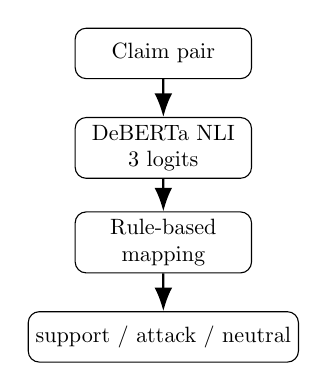
\begin{tikzpicture}[scale=0.8, every node/.style={transform shape}]
        \node[draw, rounded corners, minimum width=2.8cm, minimum height=0.8cm, align=center] (pair) at (0,0) {Claim pair};
        \node[draw, rounded corners, minimum width=2.8cm, minimum height=0.8cm, align=center] (nli) at (0,-1.5) {DeBERTa NLI\\3 logits};
        \node[draw, rounded corners, minimum width=2.8cm, minimum height=0.8cm, align=center] (rule) at (0,-3.0) {Rule-based\\mapping};
        \node[draw, rounded corners, minimum width=2.8cm, minimum height=0.8cm, align=center] (out) at (0,-4.5) {support / attack / neutral};
        \draw[-{Latex[length=3mm]}, thick] (pair) -- (nli);
        \draw[-{Latex[length=3mm]}, thick] (nli) -- (rule);
        \draw[-{Latex[length=3mm]}, thick] (rule) -- (out);
      \end{tikzpicture}
    \end{column}
  \end{columns}
\end{frame}

\begin{frame}{Experiment 1 Results and Interpretation}
Accuracy: \(0.5601\), Macro-F1: \(0.3907\), Weighted-F1: \(0.4658\)

\vspace{0.3cm}
\centering
\begin{tabular}{lccc}
\toprule
Class & Precision & Recall & F1 \\
\midrule
Support & 0.8182 & 0.1081 & 0.1910 \\
Attack & 0.8722 & 0.1742 & 0.2904 \\
Neutral & 0.5338 & 0.9790 & 0.6909 \\
\bottomrule
\end{tabular}

\vspace{0.4cm}
Interpretation:
\begin{itemize}
  \item The model is extremely conservative for support and attack
  \item It overpredicts neutral, giving high neutral recall
  \item NLI evidence alone is not sufficient for discourse stance classification
\end{itemize}
\end{frame}

\begin{frame}{Experiment 2: Old Stance Baseline}
  \begin{columns}[T]
    \begin{column}{0.56\textwidth}
      \begin{itemize}
        \item Input: source-target claim pair
        \item Model: target-dependent stance classifier
        \item Output logits: against, none, favor
        \item Final relation predicted directly from stance outputs
      \end{itemize}

      Key weakness:
      \begin{itemize}
        \item Stance specialization helps some classes
        \item But there is still no NLI fusion and no graph context
      \end{itemize}
    \end{column}
    \begin{column}{0.4\textwidth}
      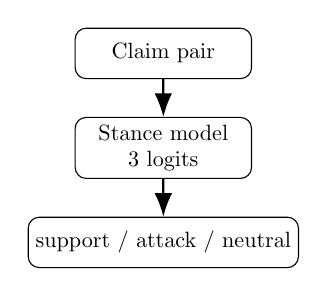
\begin{tikzpicture}[scale=0.8, every node/.style={transform shape}]
        \node[draw, rounded corners, minimum width=2.8cm, minimum height=0.8cm, align=center] (pair) at (0,0) {Claim pair};
        \node[draw, rounded corners, minimum width=2.8cm, minimum height=0.8cm, align=center] (stance) at (0,-1.5) {Stance model\\3 logits};
        \node[draw, rounded corners, minimum width=2.8cm, minimum height=0.8cm, align=center] (out) at (0,-3.0) {support / attack / neutral};
        \draw[-{Latex[length=3mm]}, thick] (pair) -- (stance);
        \draw[-{Latex[length=3mm]}, thick] (stance) -- (out);
      \end{tikzpicture}
    \end{column}
  \end{columns}
\end{frame}

\begin{frame}{Experiment 2 Results and Interpretation}
Accuracy: \(0.3517\), Macro-F1: \(0.3104\), Weighted-F1: \(0.3349\)

\vspace{0.3cm}
\centering
\begin{tabular}{lccc}
\toprule
Class & Precision & Recall & F1 \\
\midrule
Support & 0.2607 & 0.7162 & 0.3822 \\
Attack & 0.2844 & 0.0931 & 0.1403 \\
Neutral & 0.6461 & 0.2988 & 0.4086 \\
\bottomrule
\end{tabular}

\vspace{0.4cm}
Interpretation:
\begin{itemize}
  \item The stance model overpredicts support
  \item Support recall improves, but attack performance collapses
  \item The two single-model baselines fail in opposite directions
\end{itemize}
\end{frame}

\begin{frame}{Experiment 3: DeBERTa + Stance Logistic Regression}
  \begin{columns}[T]
    \begin{column}{0.58\textwidth}
      The next idea is feature fusion:
      \begin{itemize}
        \item Concatenate NLI logits and stance logits
        \item Create a 6-dimensional fused feature vector
        \item Train a multinomial logistic regression classifier
      \end{itemize}

      This baseline tests whether the two transformer models are complementary.
    \end{column}
    \begin{column}{0.38\textwidth}
      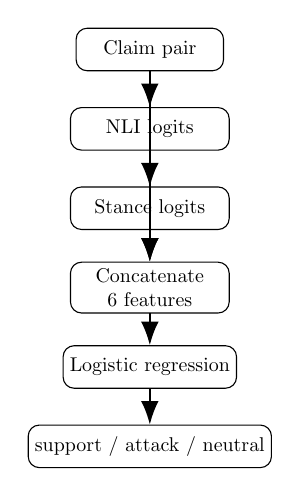
\begin{tikzpicture}[scale=0.72, every node/.style={transform shape}]
        \node[draw, rounded corners, minimum width=2.6cm, minimum height=0.75cm, align=center] (pair) at (0,0) {Claim pair};
        \node[draw, rounded corners, minimum width=2.8cm, minimum height=0.75cm, align=center] (nli) at (0,-1.4) {NLI logits};
        \node[draw, rounded corners, minimum width=2.8cm, minimum height=0.75cm, align=center] (stance) at (0,-2.8) {Stance logits};
        \node[draw, rounded corners, minimum width=2.8cm, minimum height=0.75cm, align=center] (concat) at (0,-4.2) {Concatenate\\6 features};
        \node[draw, rounded corners, minimum width=2.8cm, minimum height=0.75cm, align=center] (lr) at (0,-5.6) {Logistic regression};
        \node[draw, rounded corners, minimum width=2.8cm, minimum height=0.75cm, align=center] (out) at (0,-7.0) {support / attack / neutral};
        \draw[-{Latex[length=3mm]}, thick] (pair) -- (nli);
        \draw[-{Latex[length=3mm]}, thick] (pair) -- (stance);
        \draw[-{Latex[length=3mm]}, thick] (nli) -- (concat);
        \draw[-{Latex[length=3mm]}, thick] (stance) -- (concat);
        \draw[-{Latex[length=3mm]}, thick] (concat) -- (lr);
        \draw[-{Latex[length=3mm]}, thick] (lr) -- (out);
      \end{tikzpicture}
    \end{column}
  \end{columns}
\end{frame}

\begin{frame}{Experiment 3 Results and Interpretation}
Accuracy: \(0.6513\), Macro-F1: \(0.6557\), Weighted-F1: \(0.6477\)

\vspace{0.3cm}
\centering
\begin{tabular}{lccc}
\toprule
Class & Precision & Recall & F1 \\
\midrule
Support & 0.5726 & 0.7102 & 0.6340 \\
Attack & 0.6257 & 0.8183 & 0.7092 \\
Neutral & 0.7415 & 0.5383 & 0.6237 \\
\bottomrule
\end{tabular}

\vspace{0.4cm}
Interpretation:
\begin{itemize}
  \item This is the first genuinely balanced baseline
  \item Fusion successfully offsets the single-model biases
  \item However, classification is still pairwise and local
\end{itemize}
\end{frame}

\section{Graph-Aware Model}

\begin{frame}{Why Move Beyond Pairwise Fusion?}
The logistic-regression baseline is much stronger, but it still ignores debate-local structure.

Questions it cannot answer directly:
\begin{itemize}
  \item Is the source claim central or isolated in the debate?
  \item Does the target lie inside the source's semantic neighborhood?
  \item Do the two claims share the same semantic cluster?
  \item Is the pair locally embedded in the same debate subtopic?
\end{itemize}

The graph-aware model adds exactly this missing context.
\end{frame}

\begin{frame}[shrink=4]{Why Graph Features Matter Even Though They Are Structural}
Graph features do not replace pairwise semantics. They solve a different problem.

\vspace{0.2cm}
\begin{block}{Key Intuition}
Pairwise models answer: ``What do these two claims seem to say to each other?''\\
Graph features answer: ``Where do these two claims sit inside the local debate neighborhood?''
\end{block}

\vspace{0.2cm}
Why this matters:
\begin{itemize}
  \item Two claim pairs can look textually similar but play different discourse roles.
  \item Topical similarity alone does not tell us whether the relation is support, attack, or just same-topic neutral.
  \item Local neighborhood structure tells us whether the two claims belong to the same argumentative region, whether one is central, and whether the pair is locally important.
\end{itemize}
\end{frame}

\begin{frame}[shrink=3]{Simple Intuition for Why Graph Features Help}
Consider three claims in the same debate:
\begin{itemize}
  \item Claim A: ``Governments should subsidize renewable energy.''
  \item Claim B: ``Public funding is necessary to speed up the energy transition.''
  \item Claim C: ``Subsidies distort markets and reduce competition.''
\end{itemize}

A pairwise model sees topic overlap in all three claims because they all discuss subsidies and energy policy.

\vspace{0.2cm}
The graph-aware view adds a clearer interpretation:
\begin{itemize}
  \item A and B are likely to share neighbors and appear in the same support cluster.
  \item C may still be topically close, but it will often sit in a different neighborhood pattern and connect differently to nearby claims.
  \item Structure therefore helps separate ``same topic'' from ``same stance''.
\end{itemize}
\end{frame}

\begin{frame}{Graph-Aware Model: Core Idea}
The graph-aware model combines:
\begin{enumerate}
  \item Pairwise NLI evidence
  \item Pairwise stance evidence
  \item Debate-local semantic graph features
\end{enumerate}

This yields:
\[
\mathbf{x}_{\text{full}}
=
\left[
\mathbf{x}_{\text{NLI}} \; ; \; \mathbf{x}_{\text{stance}} \; ; \; \mathbf{x}_{\text{graph}}
\right]
\in \mathbb{R}^{13}
\]

The final classifier is a Random Forest with \(400\) trees.
\end{frame}

\begin{frame}[shrink=6]{Graph-Aware Architecture}
\centering
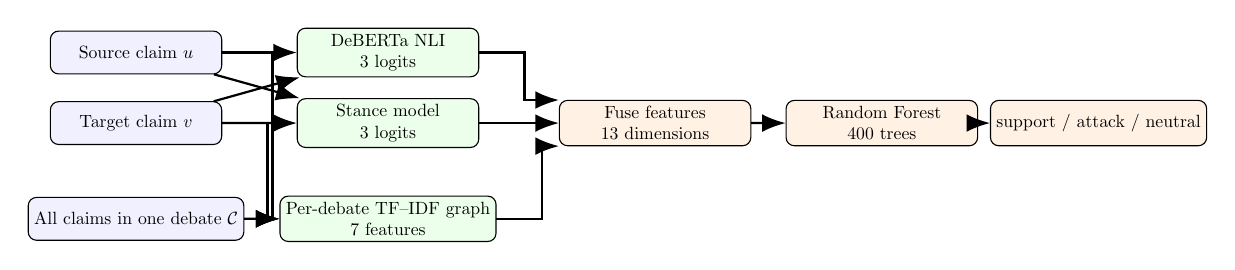
\begin{tikzpicture}[scale=0.64, every node/.style={transform shape},
  proc/.style={draw, rounded corners=3pt, minimum width=3.4cm, minimum height=0.85cm, align=center, fill=blue!6},
  feat/.style={draw, rounded corners=3pt, minimum width=3.6cm, minimum height=0.9cm, align=center, fill=green!8},
  cls/.style={draw, rounded corners=3pt, minimum width=3.8cm, minimum height=0.9cm, align=center, fill=orange!10}
]
\node[proc] (source) at (0,2.2) {Source claim \(u\)};
\node[proc] (target) at (0,0.8) {Target claim \(v\)};
\node[proc] (debate) at (0,-1.1) {All claims in one debate \(\mathcal{C}\)};

\node[feat] (nli) at (5.0,2.2) {DeBERTa NLI\\3 logits};
\node[feat] (stance) at (5.0,0.8) {Stance model\\3 logits};
\node[feat] (graph) at (5.0,-1.1) {Per-debate TF--IDF graph\\7 features};

\node[cls] (concat) at (10.3,0.8) {Fuse features\\13 dimensions};
\node[cls] (forest) at (14.8,0.8) {Random Forest\\400 trees};
\node[cls] (pred) at (19.1,0.8) {support / attack / neutral};

\draw[-{Latex[length=3mm]}, thick] (source) -- (nli);
\draw[-{Latex[length=3mm]}, thick] (target) -- (nli);
\draw[-{Latex[length=3mm]}, thick] (source) -- (stance);
\draw[-{Latex[length=3mm]}, thick] (target) -- (stance);
\draw[-{Latex[length=3mm]}, thick] (debate) -- (graph);
\draw[-{Latex[length=3mm]}, thick] (source.east) -- ++(1.0,0) |- (graph.west);
\draw[-{Latex[length=3mm]}, thick] (target.east) -- ++(0.9,0) |- (graph.west);
\draw[-{Latex[length=3mm]}, thick] (nli.east) -- ++(0.9,0) |- (concat.north west);
\draw[-{Latex[length=3mm]}, thick] (stance.east) -- (concat.west);
\draw[-{Latex[length=3mm]}, thick] (graph.east) -- ++(0.9,0) |- (concat.south west);
\draw[-{Latex[length=3mm]}, thick] (concat) -- (forest);
\draw[-{Latex[length=3mm]}, thick] (forest) -- (pred);
\end{tikzpicture}
\end{frame}

\begin{frame}[shrink=4]{Theory: Per-Debate TF--IDF Representation}
For each debate, TF--IDF is fit \emph{only on claims in that debate}.

\[
\mathrm{tf}(t,c_i) = \text{count of term } t \text{ in claim } c_i
\]
\[
\mathrm{idf}(t,\mathcal{C}) = \log\left(\frac{1 + |\mathcal{C}|}{1 + |\{c \in \mathcal{C}: t \in c\}|}\right)+1
\]
\[
\mathrm{tfidf}(t,c_i,\mathcal{C}) = \mathrm{tf}(t,c_i)\cdot \mathrm{idf}(t,\mathcal{C})
\]

Why per debate?
\begin{itemize}
  \item Topics are local to each debate.
  \item Salience should be measured within the current debate, not globally.
  \item This makes the graph features debate-sensitive rather than corpus-generic.
\end{itemize}
\end{frame}

\begin{frame}[shrink=3]{Theory: Similarity Graph Construction}
Let \(\mathbf{t}_i\) be the TF--IDF vector of claim \(c_i\). Similarity is:
\[
\mathrm{sim}(c_i,c_j)
=
\frac{\mathbf{t}_i^\top \mathbf{t}_j}{\|\mathbf{t}_i\|_2\|\mathbf{t}_j\|_2}
\]

For each claim, retain neighbors satisfying:
\begin{itemize}
  \item Cosine similarity \(\ge \tau\).
  \item Membership among the top-\(k\) neighbors.
\end{itemize}

Saved benchmark values:
\[
k = 8, \qquad \tau = 0.15
\]

This produces the local neighborhood set:
\[
N_k(c_i)
\]
\end{frame}

\begin{frame}[shrink=8]{Theory: The Seven Graph Features}
\small
\begin{enumerate}
  \item Cosine similarity: \(f_1(u,v)=\mathrm{sim}(u,v)\)
  \item Normalized source degree: \(f_2(u,v)=\frac{|N_k(u)|}{\max(1,k)}\)
  \item Normalized target degree: \(f_3(u,v)=\frac{|N_k(v)|}{\max(1,k)}\)
  \item Target-in-source: \(f_4(u,v)=\mathbf{1}[v \in N_k(u)]\)
  \item Source-in-target: \(f_5(u,v)=\mathbf{1}[u \in N_k(v)]\)
  \item Neighbor-set Jaccard overlap:
  \[
  f_6(u,v)=\frac{|N_k(u)\cap N_k(v)|}{|N_k(u)\cup N_k(v)|}
  \]
  \item Token-level Jaccard overlap:
  \[
  f_7(u,v)=\frac{|T(u)\cap T(v)|}{|T(u)\cup T(v)|}
  \]
\end{enumerate}
\normalsize
\end{frame}

\begin{frame}[shrink=8]{Feature Logic I: Degree Features}
\small
\textbf{1. Normalized source degree}
\[
f_2(u,v)=\frac{|N_k(u)|}{\max(1,k)}
\]
What problem it solves:
\begin{itemize}
  \item A claim can be very central or very isolated in the debate.
  \item Pairwise models cannot tell whether the source is broadly connected to many nearby claims.
\end{itemize}

Intuition:
\begin{itemize}
  \item High source degree often means the source is semantically broad or central.
  \item Low source degree often means the source is very specific or isolated.
\end{itemize}

Example:
\begin{itemize}
  \item If claim \(u\) is similar to many claims about ``renewable energy policy'', it is probably a central debate claim rather than a fringe statement.
\end{itemize}

\textbf{2. Normalized target degree}
\[
f_3(u,v)=\frac{|N_k(v)|}{\max(1,k)}
\]
This solves the same problem for the target. It helps the model know whether the target is a core motion claim or a peripheral claim.
\normalsize
\end{frame}

\begin{frame}[shrink=8]{Feature Logic II: Neighborhood Membership Features}
\small
\textbf{3. Target-in-source}
\[
f_4(u,v)=\mathbf{1}[v \in N_k(u)]
\]
What problem it solves:
\begin{itemize}
  \item Cosine similarity alone tells us how similar two claims are.
  \item It does not tell us whether that similarity is strong enough to make the target one of the source's \emph{important local neighbors}.
\end{itemize}

Example:
\begin{itemize}
  \item If \(u\) says ``Subsidize renewables now'' and \(v\) says ``Government should fund clean energy'', then \(v\) may be one of the strongest semantic anchors for \(u\).
\end{itemize}

\textbf{4. Source-in-target}
\[
f_5(u,v)=\mathbf{1}[u \in N_k(v)]
\]
Why it matters:
\begin{itemize}
  \item Neighborhood structure is directed.
  \item \(v\) may be a strong neighbor of \(u\), but \(u\) may not be a strong neighbor of \(v\).
  \item This asymmetry captures specificity vs generality.
\end{itemize}
\normalsize
\end{frame}

\begin{frame}[shrink=8]{Feature Logic III: Overlap Features}
\small
\textbf{5. Neighbor-set Jaccard overlap}
\[
f_6(u,v)=\frac{|N_k(u)\cap N_k(v)|}{|N_k(u)\cup N_k(v)|}
\]
What problem it solves:
\begin{itemize}
  \item Two claims may not directly be nearest neighbors.
  \item They may still live in the same local semantic region of the debate.
\end{itemize}

Example:
\begin{itemize}
  \item One claim talks about emissions, another about renewable subsidies.
  \item If both connect to the same cluster of climate-policy claims, they likely belong to the same argumentative neighborhood.
\end{itemize}

\textbf{6. Token-level Jaccard overlap}
\[
f_7(u,v)=\frac{|T(u)\cap T(v)|}{|T(u)\cup T(v)|}
\]
What problem it solves:
\begin{itemize}
  \item TF--IDF can miss simple literal reuse patterns.
  \item Token overlap recovers cases where two claims share key surface words or phrases.
\end{itemize}
\normalsize
\end{frame}

\begin{frame}[shrink=5]{Feature Logic IV: Why These Features Work Together}
\small
Each graph feature solves a different weakness of pure pairwise prediction:
\begin{itemize}
  \item \textbf{Degree features} tell us whether the source and target are central or peripheral.
  \item \textbf{Membership features} tell us whether the pair is locally important in each other's neighborhood.
  \item \textbf{Overlap features} tell us whether the two claims belong to the same local semantic region.
\end{itemize}

Why this is better than just cosine similarity:
\begin{itemize}
  \item Cosine similarity is only one local number.
  \item The debate graph needs structure: centrality, asymmetry, and neighborhood overlap.
  \item These features let the model reason about context without building a full GNN.
\end{itemize}

This is why the graph-aware model is not just ``pairwise model + one similarity score''. It is a structured local-context model.
\normalsize
\end{frame}

\begin{frame}[shrink=3]{Why Use a Random Forest?}
The final classifier receives a 13-dimensional fused representation.

Random Forest is used because:
\begin{itemize}
  \item The 6 transformer logits are useful but not fully linear.
  \item The graph features create thresholded and interaction-heavy patterns.
  \item Tree ensembles can capture nonlinear combinations naturally.
\end{itemize}

Prediction rule:
\[
\hat{\mathbf{p}}(\mathbf{x}) = \frac{1}{M}\sum_{m=1}^{M} T_m(\mathbf{x}), \qquad M=400
\]
\[
\hat{y} = \arg\max_c \hat{p}_c(\mathbf{x})
\]
\end{frame}

\begin{frame}[shrink=4]{Graph-Aware Training Protocol}
\begin{enumerate}
  \item Load debate graphs.
  \item Parse gold support and attack edges.
  \item Sample neutral non-edges.
  \item Split debates into train and test by debate, not by row.
  \item Compute 6 transformer features.
  \item Compute 7 graph features within each debate.
  \item Concatenate into 13-dimensional vectors.
  \item Train Random Forest on train debates only.
  \item Evaluate on held-out debates.
\end{enumerate}
\end{frame}

\begin{frame}[shrink=3]{Graph-Aware Example: Why Local Context Helps}
  \begin{columns}[T]
    \begin{column}{0.53\textwidth}
      Suppose we want to classify the edge from:
      \begin{itemize}
        \item Source: ``Subsidize renewables to accelerate adoption''
        \item Target: ``Policy should balance costs and benefits''
      \end{itemize}

      A pairwise model only sees the two sentences.

      A graph-aware model also asks:
      \begin{itemize}
        \item Is the source central in the renewable-energy cluster?
        \item Is the target one of the source's closest semantic anchors?
        \item Do they share the same climate-policy neighborhood?
      \end{itemize}

      That extra context makes support vs attack vs neutral much easier.
    \end{column}
    \begin{column}{0.42\textwidth}
      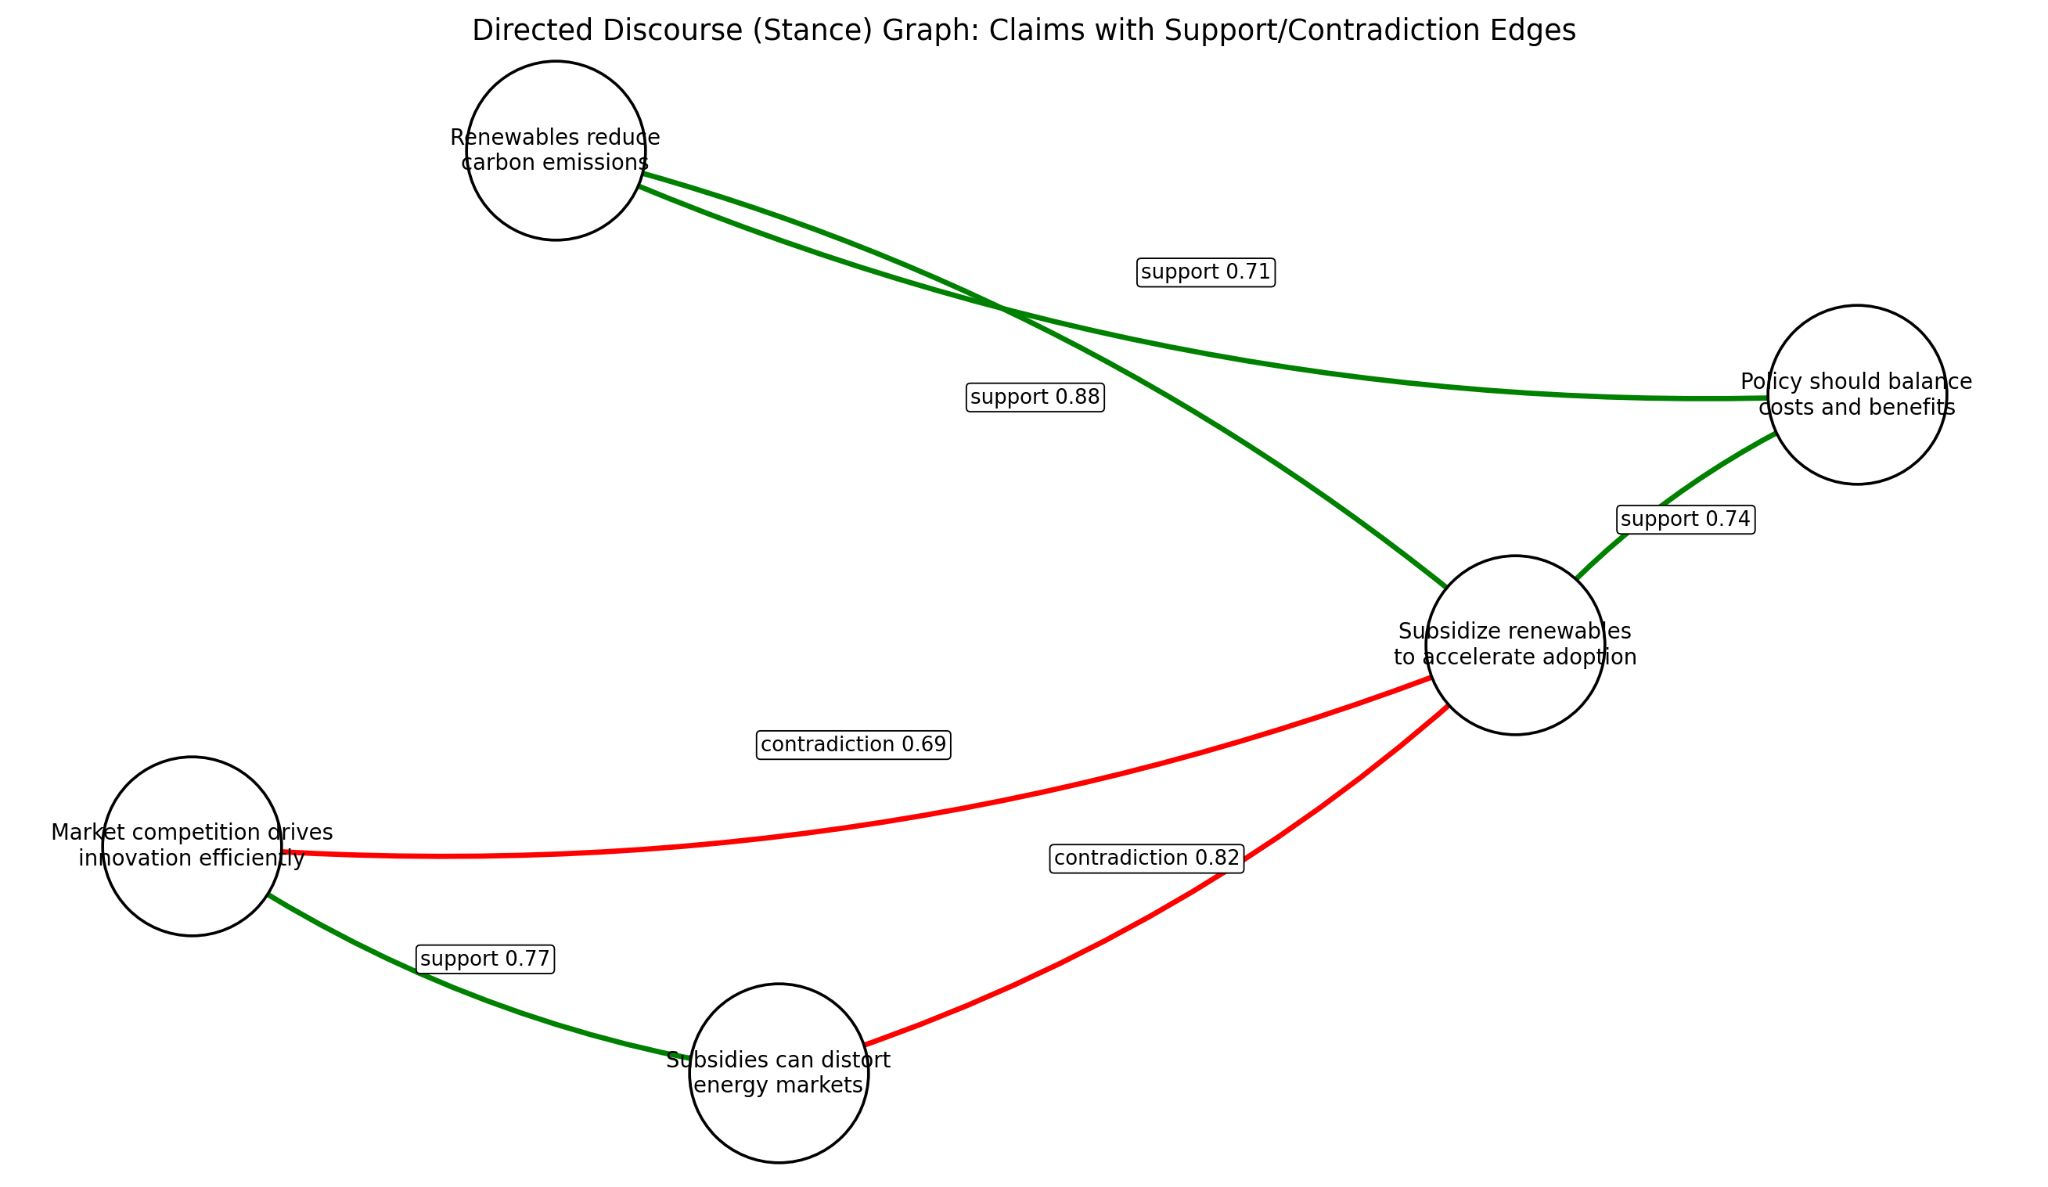
\includegraphics[width=\linewidth]{5.jpg}
    \end{column}
  \end{columns}
\end{frame}

\section{Results and Interpretation}

\begin{frame}{Aggregate Results Across All Models}
\centering
\begin{tabular}{lccc}
\toprule
Model & Accuracy & Macro-F1 & Weighted-F1 \\
\midrule
DeBERTa baseline & 0.5601 & 0.3907 & 0.4658 \\
Stance baseline & 0.3517 & 0.3104 & 0.3349 \\
DeBERTa + stance LR & 0.6513 & 0.6557 & 0.6477 \\
\textbf{Graph-aware} & \textbf{0.8818} & \textbf{0.8665} & \textbf{0.8811} \\
\bottomrule
\end{tabular}
\end{frame}

\begin{frame}{Metric Comparison Figure}
\centering
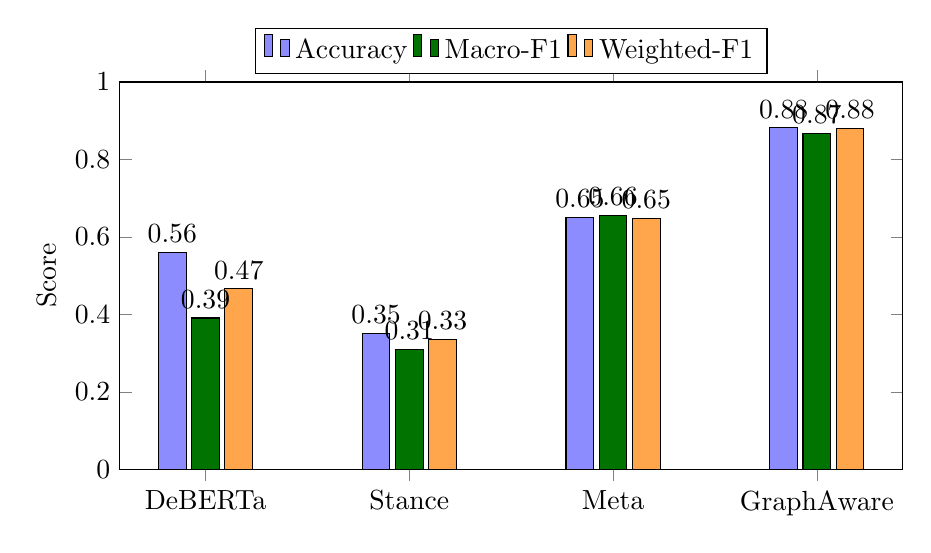
\begin{tikzpicture}
\begin{axis}[
    ybar,
    bar width=10pt,
    width=0.95\textwidth,
    height=6.5cm,
    ymin=0,
    ymax=1.0,
    ylabel={Score},
    symbolic x coords={DeBERTa,Stance,Meta,GraphAware},
    xtick=data,
    legend style={at={(0.5,1.02)}, anchor=south, legend columns=3},
    nodes near coords,
    nodes near coords align={vertical},
    enlarge x limits=0.14
]
\addplot[fill=blue!45] coordinates {(DeBERTa,0.5601) (Stance,0.3517) (Meta,0.6513) (GraphAware,0.8818)};
\addplot[fill=green!45!black] coordinates {(DeBERTa,0.3907) (Stance,0.3104) (Meta,0.6557) (GraphAware,0.8665)};
\addplot[fill=orange!70] coordinates {(DeBERTa,0.4658) (Stance,0.3349) (Meta,0.6477) (GraphAware,0.8811)};
\legend{Accuracy, Macro-F1, Weighted-F1}
\end{axis}
\end{tikzpicture}
\end{frame}

\begin{frame}{Benchmark Screens from Added Assets}
  \begin{columns}[T]
    \begin{column}{0.32\textwidth}
      \centering
      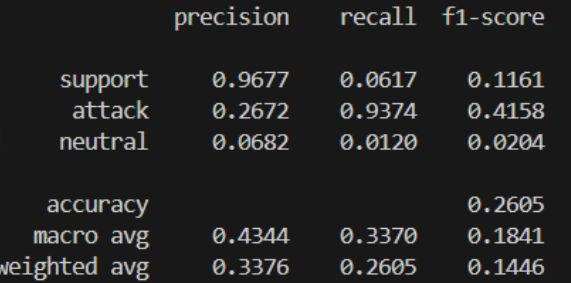
\includegraphics[width=\linewidth]{10.jpg}
      \vspace{0.15cm}

      \small DeBERTa rule baseline
    \end{column}
    \begin{column}{0.32\textwidth}
      \centering
      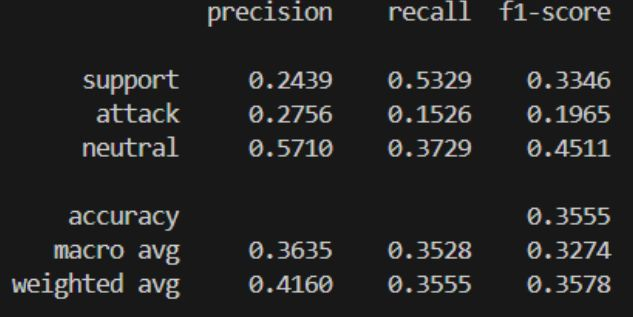
\includegraphics[width=\linewidth]{11.jpg}
      \vspace{0.15cm}

      \small stance-only baseline
    \end{column}
    \begin{column}{0.32\textwidth}
      \centering
      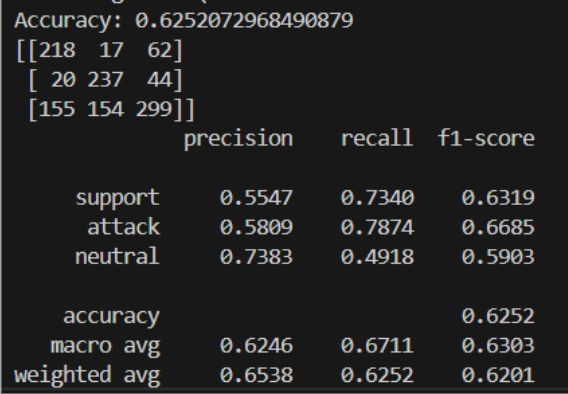
\includegraphics[width=\linewidth]{12.jpg}
      \vspace{0.15cm}

      \small fused DeBERTa + stance LR
    \end{column}
  \end{columns}
\end{frame}

\begin{frame}{Per-Class Results of the Graph-Aware Model}
\centering
\begin{tabular}{lccc}
\toprule
Class & Precision & Recall & F1 \\
\midrule
Support & 0.8485 & 0.8243 & 0.8363 \\
Attack & 0.8525 & 0.8243 & 0.8382 \\
Neutral & 0.9111 & 0.9392 & 0.9250 \\
\bottomrule
\end{tabular}

\vspace{0.5cm}
Interpretation:
\begin{itemize}
  \item Performance is strong across all three classes.
  \item Support and attack are no longer badly imbalanced.
  \item Neutral remains strong without overwhelming the other two classes.
\end{itemize}
\end{frame}

\begin{frame}[shrink=4]{Confusion Matrix Comparison I}
\centering
\begin{columns}[T]
  \begin{column}{0.48\textwidth}
    \centering
    \textbf{DeBERTa baseline}

    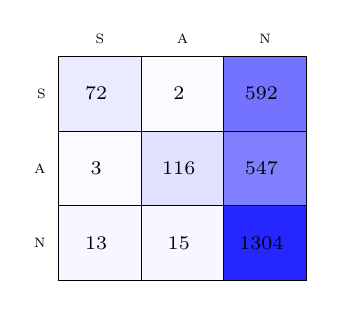
\begin{tikzpicture}[scale=0.7, every node/.style={transform shape}]
      \matrix[matrix of nodes,
      nodes={draw, minimum width=1.05cm, minimum height=0.95cm, align=center, font=\scriptsize},
      row sep=-\pgflinewidth, column sep=-\pgflinewidth] (m) {
      |[fill=blue!8]|72 & |[fill=blue!2]|2 & |[fill=blue!55]|592 \\
      |[fill=blue!2]|3 & |[fill=blue!12]|116 & |[fill=blue!50]|547 \\
      |[fill=blue!3]|13 & |[fill=blue!3]|15 & |[fill=blue!85]|1304 \\
      };
      \node[above=0.1cm of m-1-1] {\scriptsize S};
      \node[above=0.1cm of m-1-2] {\scriptsize A};
      \node[above=0.1cm of m-1-3] {\scriptsize N};
      \node[left=0.1cm of m-1-1] {\scriptsize S};
      \node[left=0.1cm of m-2-1] {\scriptsize A};
      \node[left=0.1cm of m-3-1] {\scriptsize N};
    \end{tikzpicture}

    \vspace{0.1cm}

    \scriptsize Strong neutral bias. Most support and attack examples collapse into neutral.
  \end{column}
  \begin{column}{0.48\textwidth}
    \centering
    \textbf{Stance baseline}

    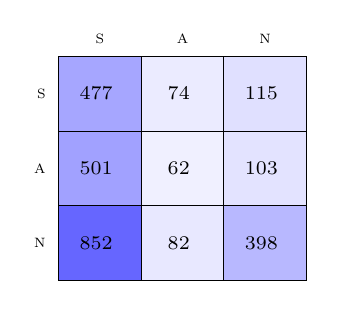
\begin{tikzpicture}[scale=0.7, every node/.style={transform shape}]
      \matrix[matrix of nodes,
      nodes={draw, minimum width=1.05cm, minimum height=0.95cm, align=center, font=\scriptsize},
      row sep=-\pgflinewidth, column sep=-\pgflinewidth] (m) {
      |[fill=blue!35]|477 & |[fill=blue!8]|74 & |[fill=blue!12]|115 \\
      |[fill=blue!37]|501 & |[fill=blue!6]|62 & |[fill=blue!11]|103 \\
      |[fill=blue!60]|852 & |[fill=blue!9]|82 & |[fill=blue!28]|398 \\
      };
      \node[above=0.1cm of m-1-1] {\scriptsize S};
      \node[above=0.1cm of m-1-2] {\scriptsize A};
      \node[above=0.1cm of m-1-3] {\scriptsize N};
      \node[left=0.1cm of m-1-1] {\scriptsize S};
      \node[left=0.1cm of m-2-1] {\scriptsize A};
      \node[left=0.1cm of m-3-1] {\scriptsize N};
    \end{tikzpicture}

    \vspace{0.1cm}

    \scriptsize Strong support bias. The model pulls many attack and neutral examples toward support.
  \end{column}
\end{columns}
\vspace{0.2cm}
\small Rows are gold labels and columns are predicted labels. Abbreviations: S = Support, A = Attack, N = Neutral.
\end{frame}

\begin{frame}[shrink=4]{Confusion Matrix Comparison II}
\centering
\begin{columns}[T]
  \begin{column}{0.48\textwidth}
    \centering
    \textbf{DeBERTa + stance LR}

    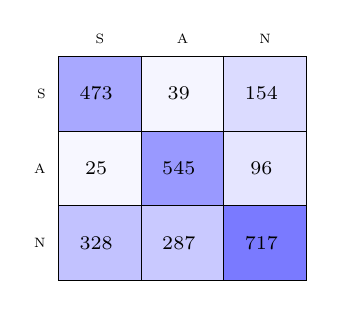
\begin{tikzpicture}[scale=0.7, every node/.style={transform shape}]
      \matrix[matrix of nodes,
      nodes={draw, minimum width=1.05cm, minimum height=0.95cm, align=center, font=\scriptsize},
      row sep=-\pgflinewidth, column sep=-\pgflinewidth] (m) {
      |[fill=blue!34]|473 & |[fill=blue!4]|39 & |[fill=blue!14]|154 \\
      |[fill=blue!3]|25 & |[fill=blue!40]|545 & |[fill=blue!10]|96 \\
      |[fill=blue!24]|328 & |[fill=blue!21]|287 & |[fill=blue!52]|717 \\
      };
      \node[above=0.1cm of m-1-1] {\scriptsize S};
      \node[above=0.1cm of m-1-2] {\scriptsize A};
      \node[above=0.1cm of m-1-3] {\scriptsize N};
      \node[left=0.1cm of m-1-1] {\scriptsize S};
      \node[left=0.1cm of m-2-1] {\scriptsize A};
      \node[left=0.1cm of m-3-1] {\scriptsize N};
    \end{tikzpicture}

    \vspace{0.1cm}

    \scriptsize Better balance than the single-model baselines, but many neutral cases are still confused with support and attack.
  \end{column}
  \begin{column}{0.48\textwidth}
    \centering
    \textbf{Graph-aware}

    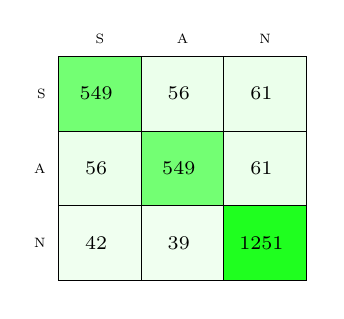
\begin{tikzpicture}[scale=0.7, every node/.style={transform shape}]
      \matrix[matrix of nodes,
      nodes={draw, minimum width=1.05cm, minimum height=0.95cm, align=center, font=\scriptsize},
      row sep=-\pgflinewidth, column sep=-\pgflinewidth] (m) {
      |[fill=green!55]|549 & |[fill=green!8]|56 & |[fill=green!8]|61 \\
      |[fill=green!8]|56 & |[fill=green!55]|549 & |[fill=green!8]|61 \\
      |[fill=green!6]|42 & |[fill=green!6]|39 & |[fill=green!88]|1251 \\
      };
      \node[above=0.1cm of m-1-1] {\scriptsize S};
      \node[above=0.1cm of m-1-2] {\scriptsize A};
      \node[above=0.1cm of m-1-3] {\scriptsize N};
      \node[left=0.1cm of m-1-1] {\scriptsize S};
      \node[left=0.1cm of m-2-1] {\scriptsize A};
      \node[left=0.1cm of m-3-1] {\scriptsize N};
    \end{tikzpicture}

    \vspace{0.1cm}

    \scriptsize Clean diagonal across all three classes. Structural context reduces both neutral confusion and support-attack cross-talk.
  \end{column}
\end{columns}

\vspace{0.25cm}
\small Rows are gold labels and columns are predicted labels. Darker cells indicate larger counts.
\end{frame}

\begin{frame}{Interpretation of the Graph-Aware Gains}
Why does the graph-aware model help so much?
\begin{enumerate}
  \item Debate-local context reduces ambiguity.
  \item Graph features separate true neutral non-edges more effectively.
  \item Semantic neighborhood overlap adds structure not available to pairwise models.
  \item Nonlinear interactions between transformer evidence and graph signals matter.
\end{enumerate}

Compared to the DeBERTa + stance logistic regression baseline:
\[
\Delta \text{Accuracy} \approx 0.2305
\]
\[
\Delta \text{Macro-F1} \approx 0.2108
\]
\end{frame}

\section{Graph Algorithms}

\begin{frame}{Why Graph Algorithms Matter After Stance Prediction}
Once stance edges are reliable, the graph becomes meaningful enough for discourse analysis.

These algorithms answer different questions:
\begin{itemize}
  \item Which claims are globally well-supported?
  \item Which claims are globally attacked?
  \item Which nodes are bottlenecks in the support structure?
  \item Which claims form coherent topical clusters?
  \item Where do contradiction paths and cycles appear?
\end{itemize}
\end{frame}

\begin{frame}{Graph Algorithm: Contradiction and Cycle Detection}
  \begin{columns}[T]
    \begin{column}{0.48\textwidth}
      Goal:
      \begin{itemize}
        \item Find explicit contradiction edges.
        \item Find directed cycles that indicate circular reasoning.
      \end{itemize}

      Why useful:
      \begin{itemize}
        \item Contradiction edges expose direct conflict.
        \item Cycles expose reasoning loops across multiple claims.
      \end{itemize}
    \end{column}
    \begin{column}{0.48\textwidth}
      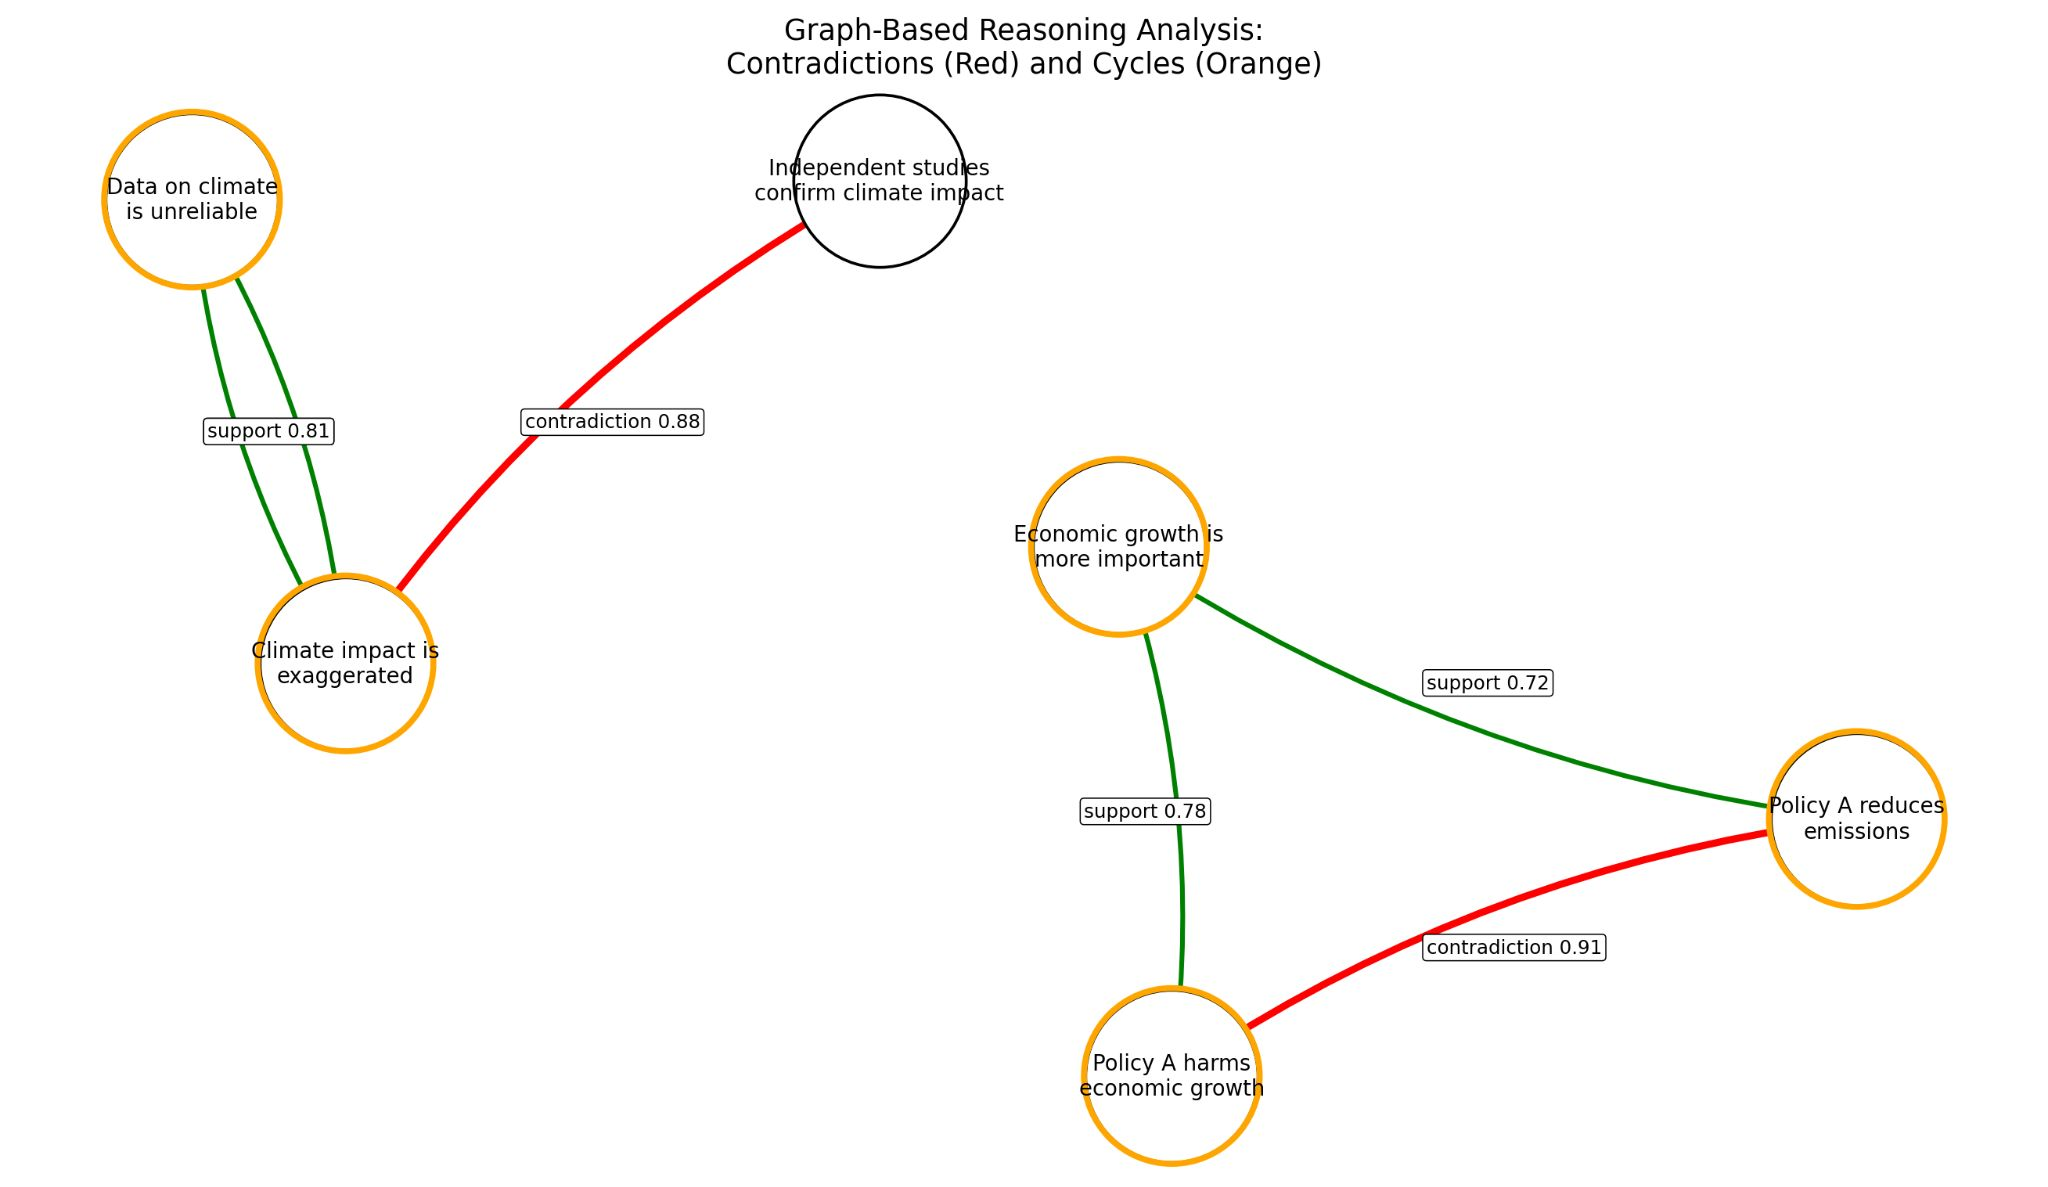
\includegraphics[width=\linewidth]{6.jpg}
    \end{column}
  \end{columns}
\end{frame}

\begin{frame}{Graph Algorithm: Support In-Degree}
  \begin{columns}[T]
    \begin{column}{0.52\textwidth}
      Idea:
      \begin{itemize}
        \item Count how many support edges point into each claim.
      \end{itemize}

      What problem it solves:
      \begin{itemize}
        \item Gives a simple measure of local support strength.
        \item Helps identify weakly supported claims.
      \end{itemize}

      Limitation:
      \begin{itemize}
        \item Only local, and does not know whether the supporting claims are themselves important.
      \end{itemize}
    \end{column}
    \begin{column}{0.43\textwidth}
      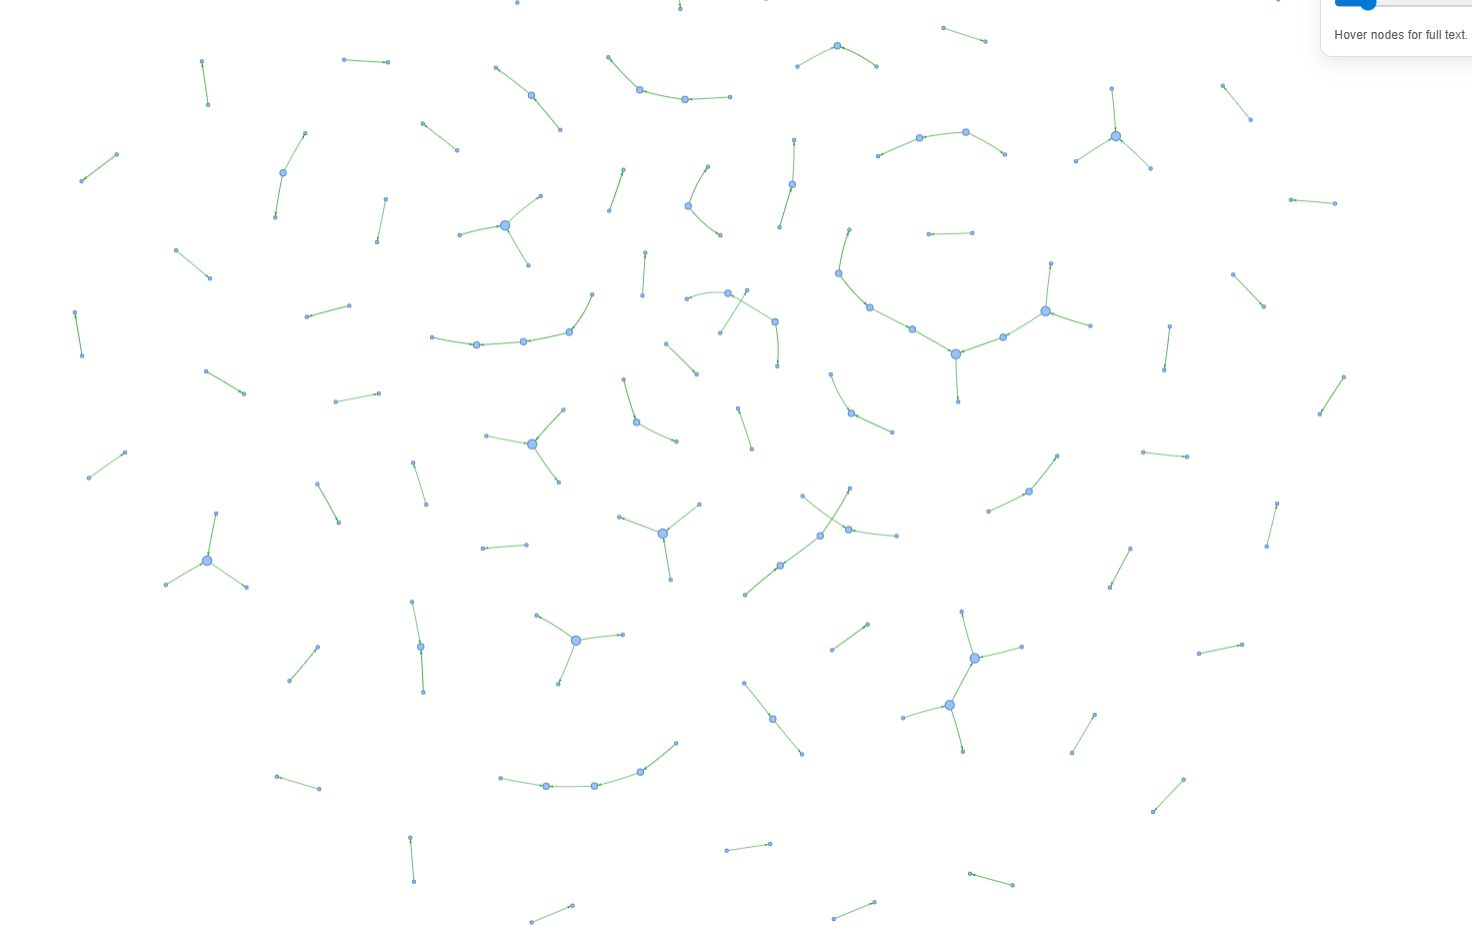
\includegraphics[width=\linewidth]{15.jpg}
    \end{column}
  \end{columns}
\end{frame}

\begin{frame}{Graph Algorithm: PageRank on the Support Graph}
  \begin{columns}[T]
    \begin{column}{0.5\textwidth}
      Goal:
      \begin{itemize}
        \item Rank claims by global support influence.
      \end{itemize}

      Logic:
      \begin{itemize}
        \item A claim is important if it is supported by other important claims.
      \end{itemize}

      Why better than in-degree:
      \begin{itemize}
        \item Not all supporting claims should count equally.
      \end{itemize}
    \end{column}
    \begin{column}{0.46\textwidth}
      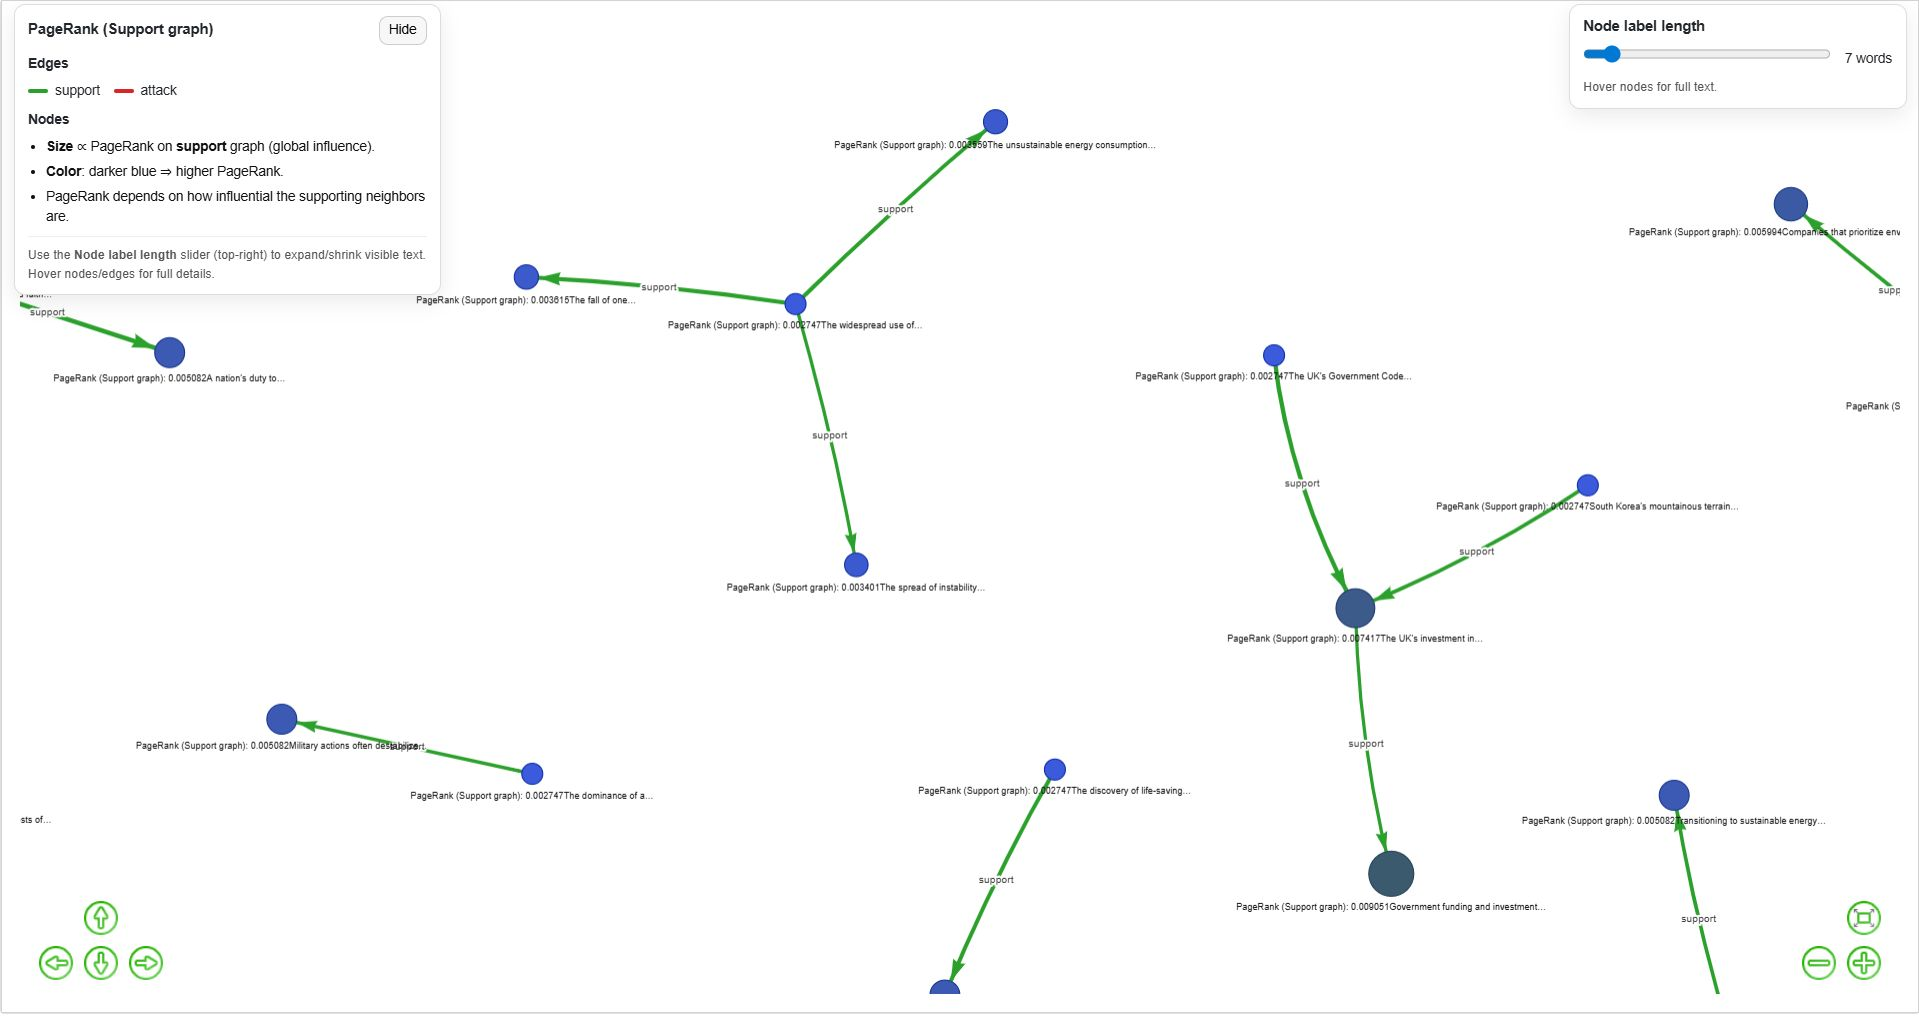
\includegraphics[width=\linewidth]{19.jpg}
    \end{column}
  \end{columns}
\end{frame}

\begin{frame}{Graph Algorithm: PageRank on the Attack Graph}
  \begin{columns}[T]
    \begin{column}{0.5\textwidth}
      Goal:
      \begin{itemize}
        \item Rank claims by global attack influence.
      \end{itemize}

      Interpretation:
      \begin{itemize}
        \item A node with high attack PageRank is attacked by influential attack pathways.
        \item This helps identify globally controversial or vulnerable claims.
      \end{itemize}
    \end{column}
    \begin{column}{0.46\textwidth}
      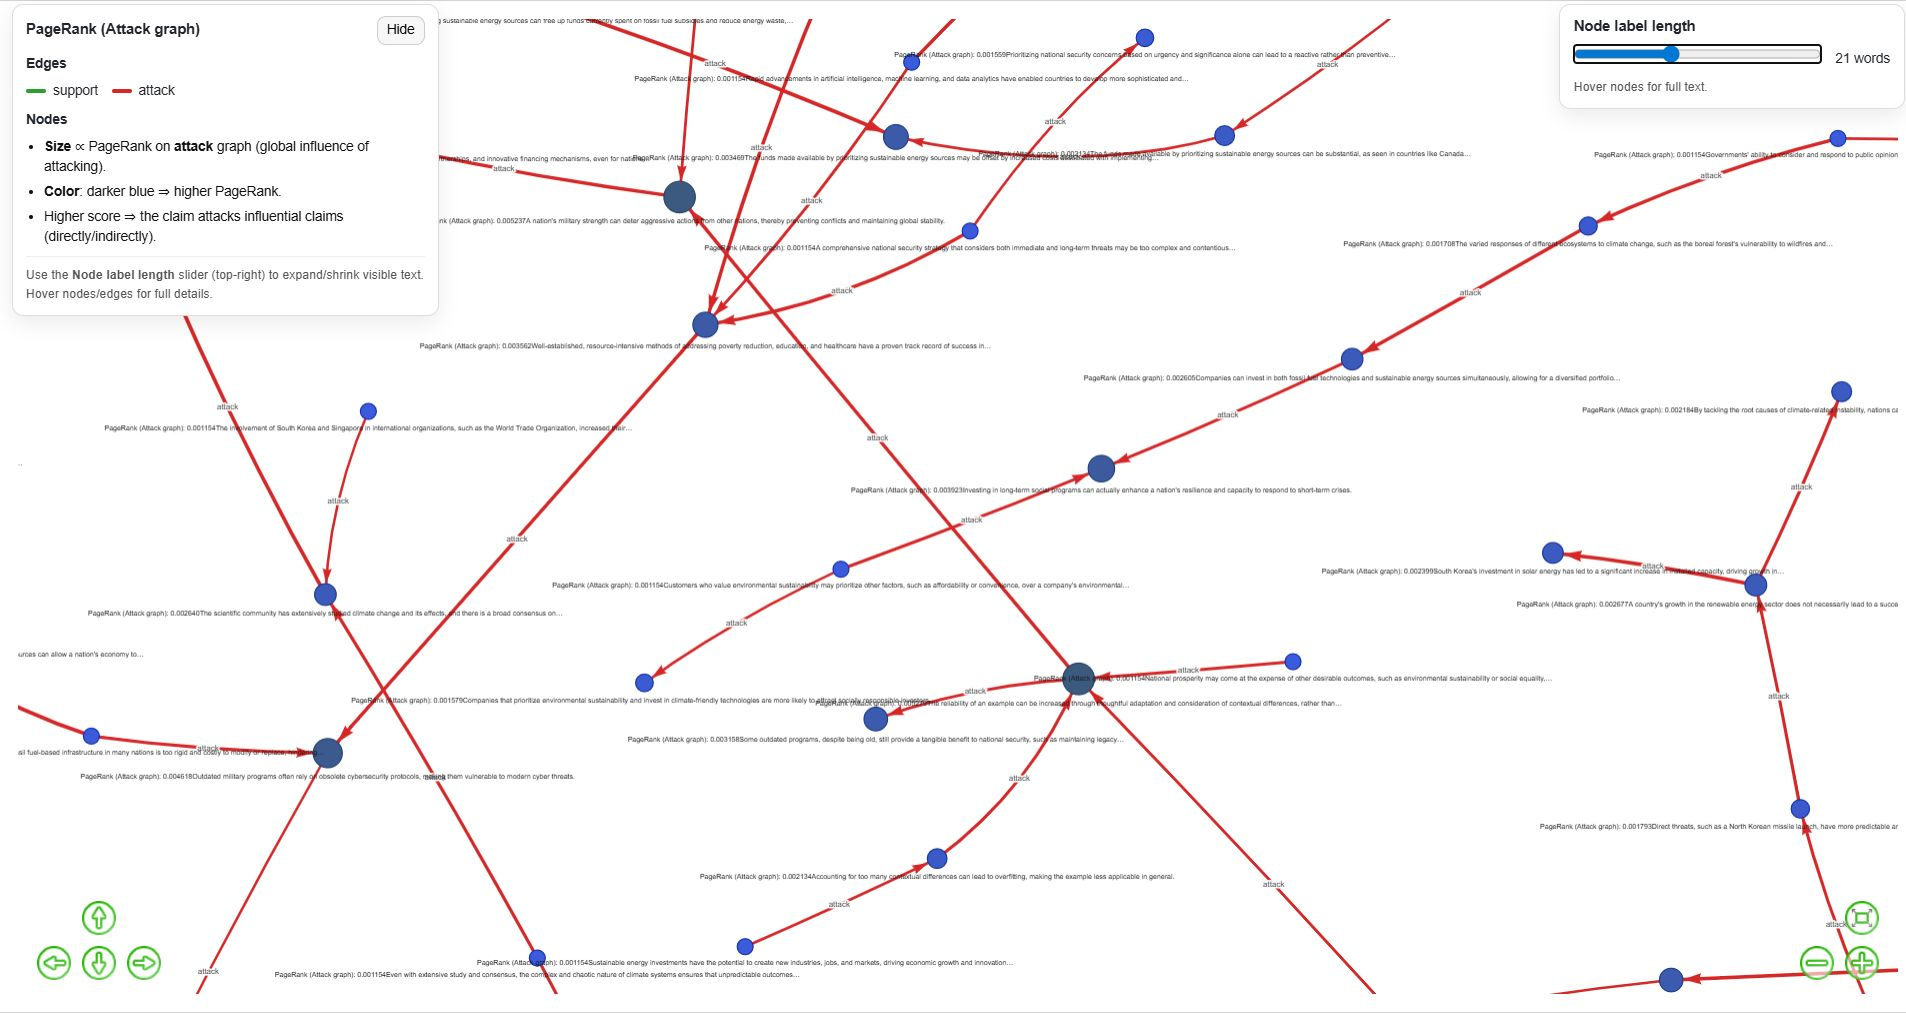
\includegraphics[width=\linewidth]{20.jpg}
    \end{column}
  \end{columns}
\end{frame}

\begin{frame}{Graph Algorithm: Net Influence}
  \begin{columns}[T]
    \begin{column}{0.5\textwidth}
      We compute:
      \[
      \text{Net Influence}(u)=PR_{\text{support}}(u)-PR_{\text{attack}}(u)
      \]

      Why this helps:
      \begin{itemize}
        \item Support and attack can both be globally strong.
        \item This score summarizes whether a claim is overall defended or challenged.
      \end{itemize}
    \end{column}
    \begin{column}{0.46\textwidth}
      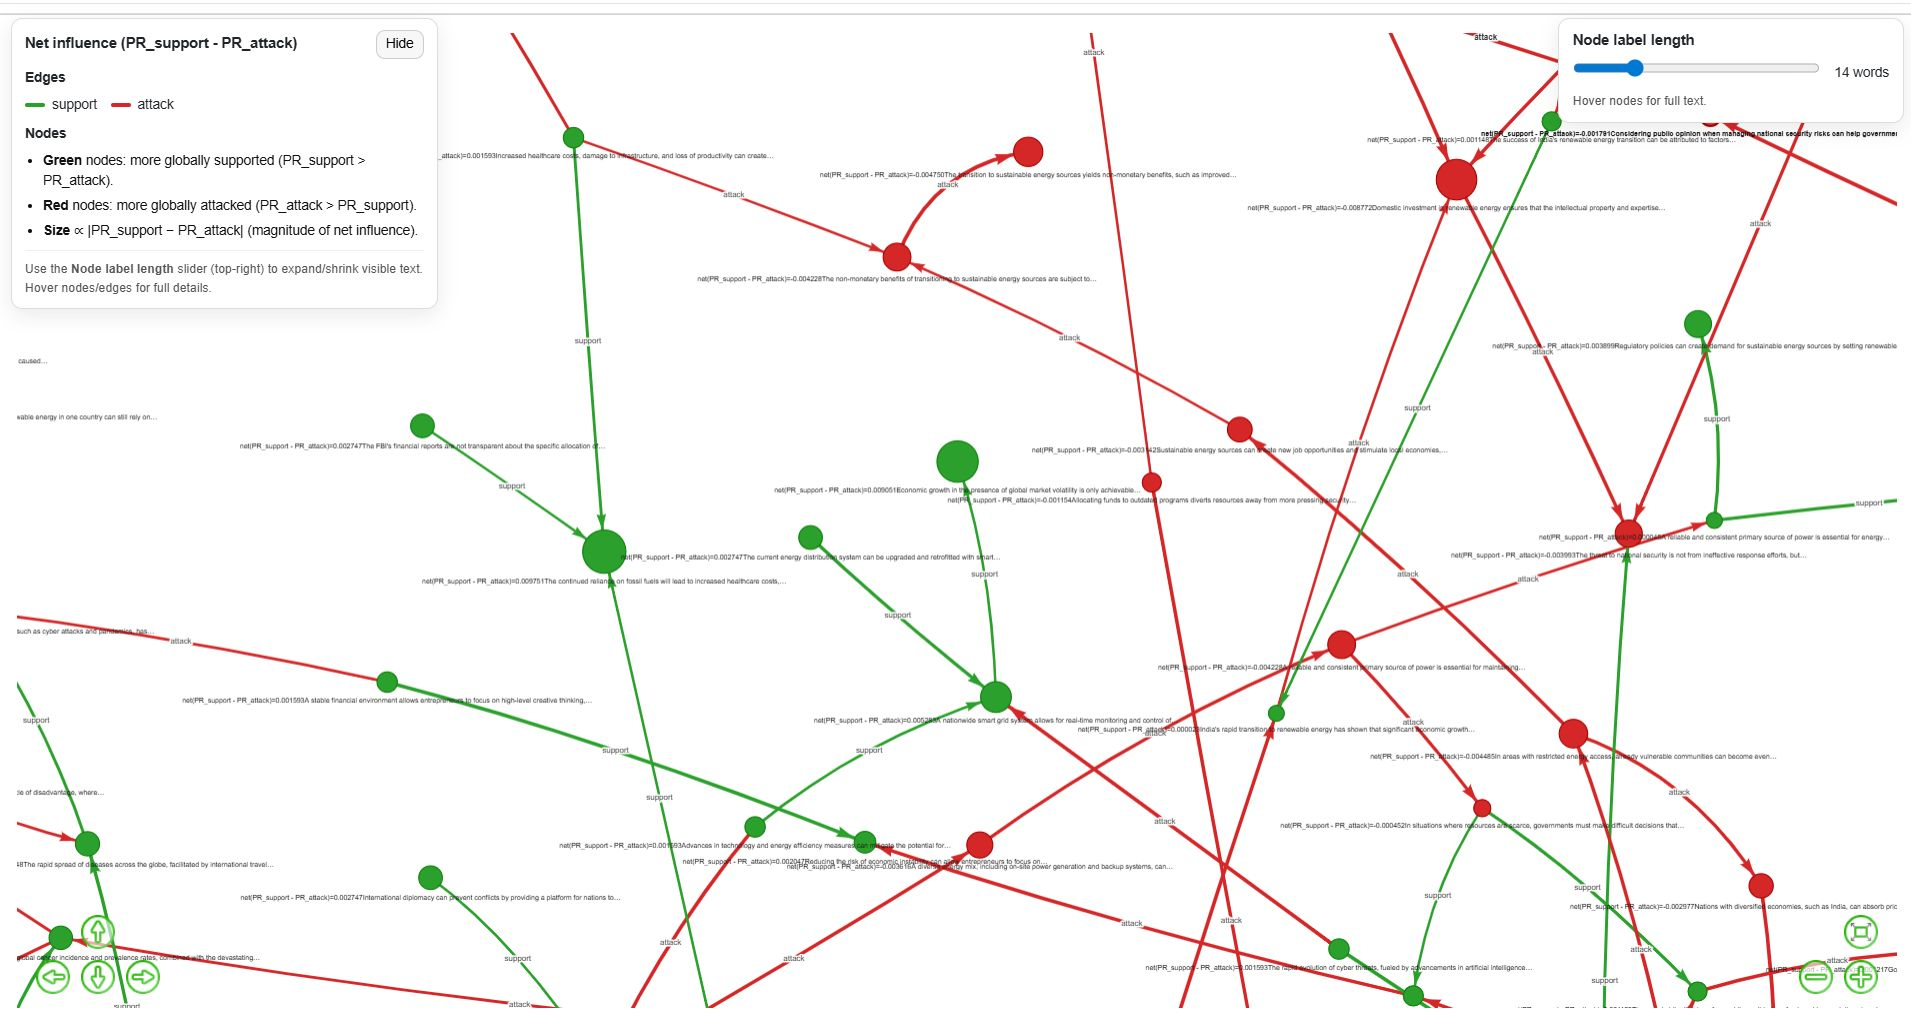
\includegraphics[width=\linewidth]{21.jpg}
    \end{column}
  \end{columns}
\end{frame}

\begin{frame}{Graph Algorithm: Min-Cut Vulnerability}
  \begin{columns}[T]
    \begin{column}{0.5\textwidth}
      Goal:
      \begin{itemize}
        \item Find bottleneck claims and weak links inside a support structure.
      \end{itemize}

      Interpretation:
      \begin{itemize}
        \item If a small cut can break a support cluster, the argument is structurally fragile.
        \item This is useful for finding vulnerable subarguments.
      \end{itemize}
    \end{column}
    \begin{column}{0.46\textwidth}
      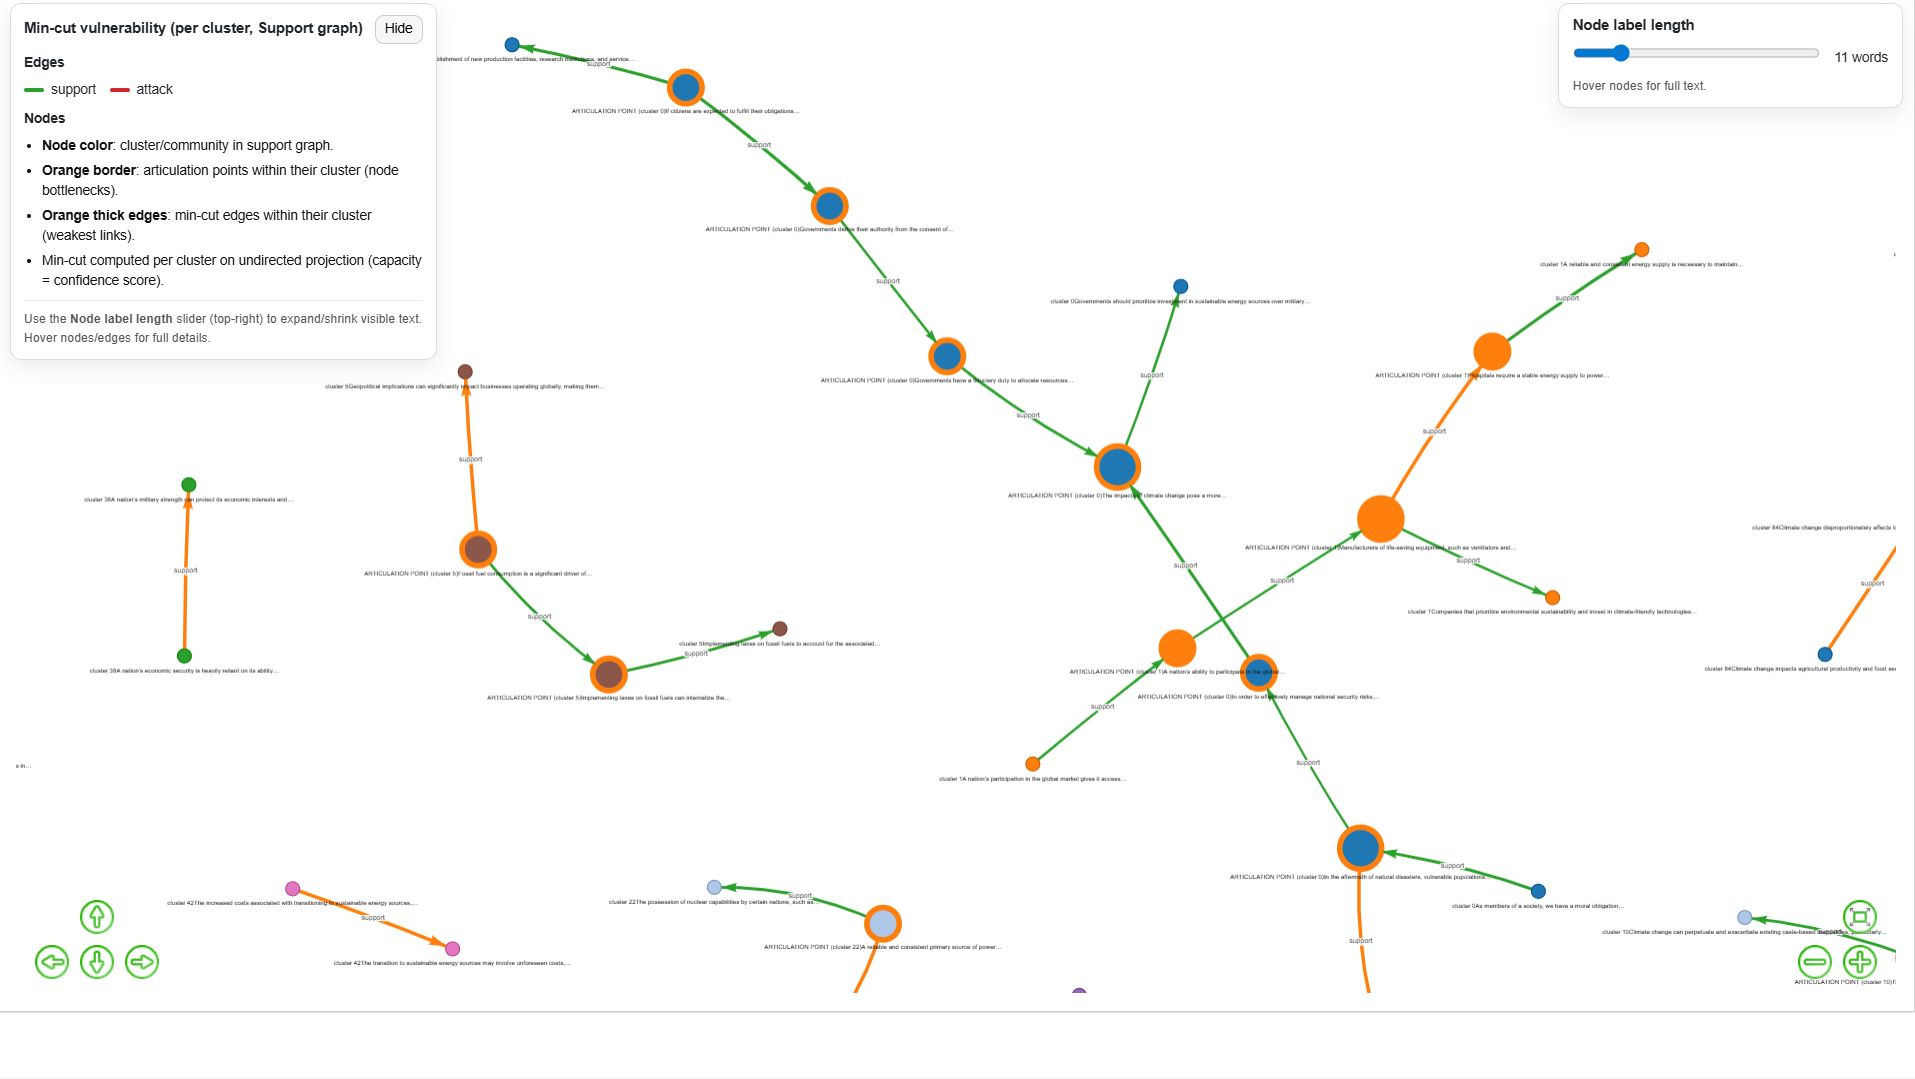
\includegraphics[width=\linewidth]{22.jpg}
    \end{column}
  \end{columns}
\end{frame}

\begin{frame}{Graph Algorithm: Clustering and Themes}
  \begin{columns}[T]
    \begin{column}{0.5\textwidth}
      Goal:
      \begin{itemize}
        \item Group claims into coherent support communities.
      \end{itemize}

      What it solves:
      \begin{itemize}
        \item Large debates often contain multiple subtopics.
        \item Clustering helps reveal local themes and debate substructures.
      \end{itemize}
    \end{column}
    \begin{column}{0.46\textwidth}
      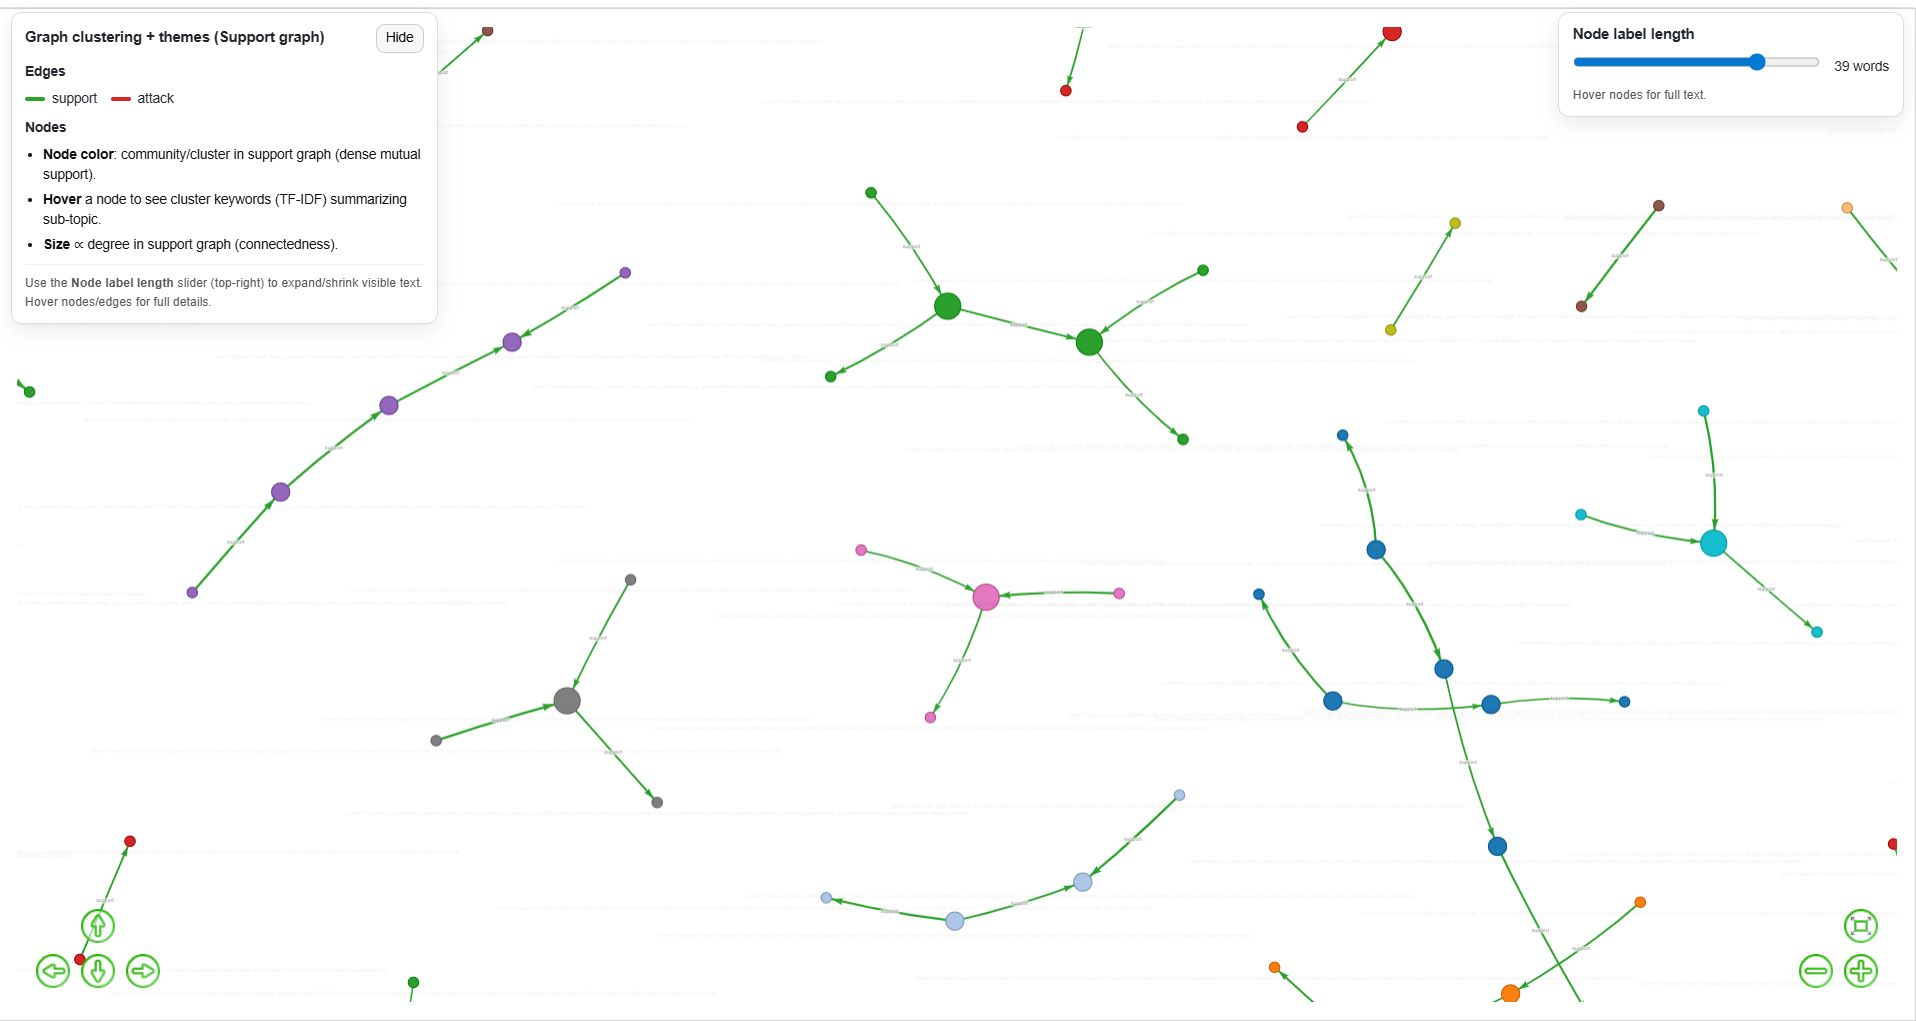
\includegraphics[width=\linewidth]{23.jpg}
    \end{column}
  \end{columns}
\end{frame}

\section{Qualitative Graphs and Legacy Figures}

\begin{frame}{Generated Stance Graph from Earlier Presentation}
\centering
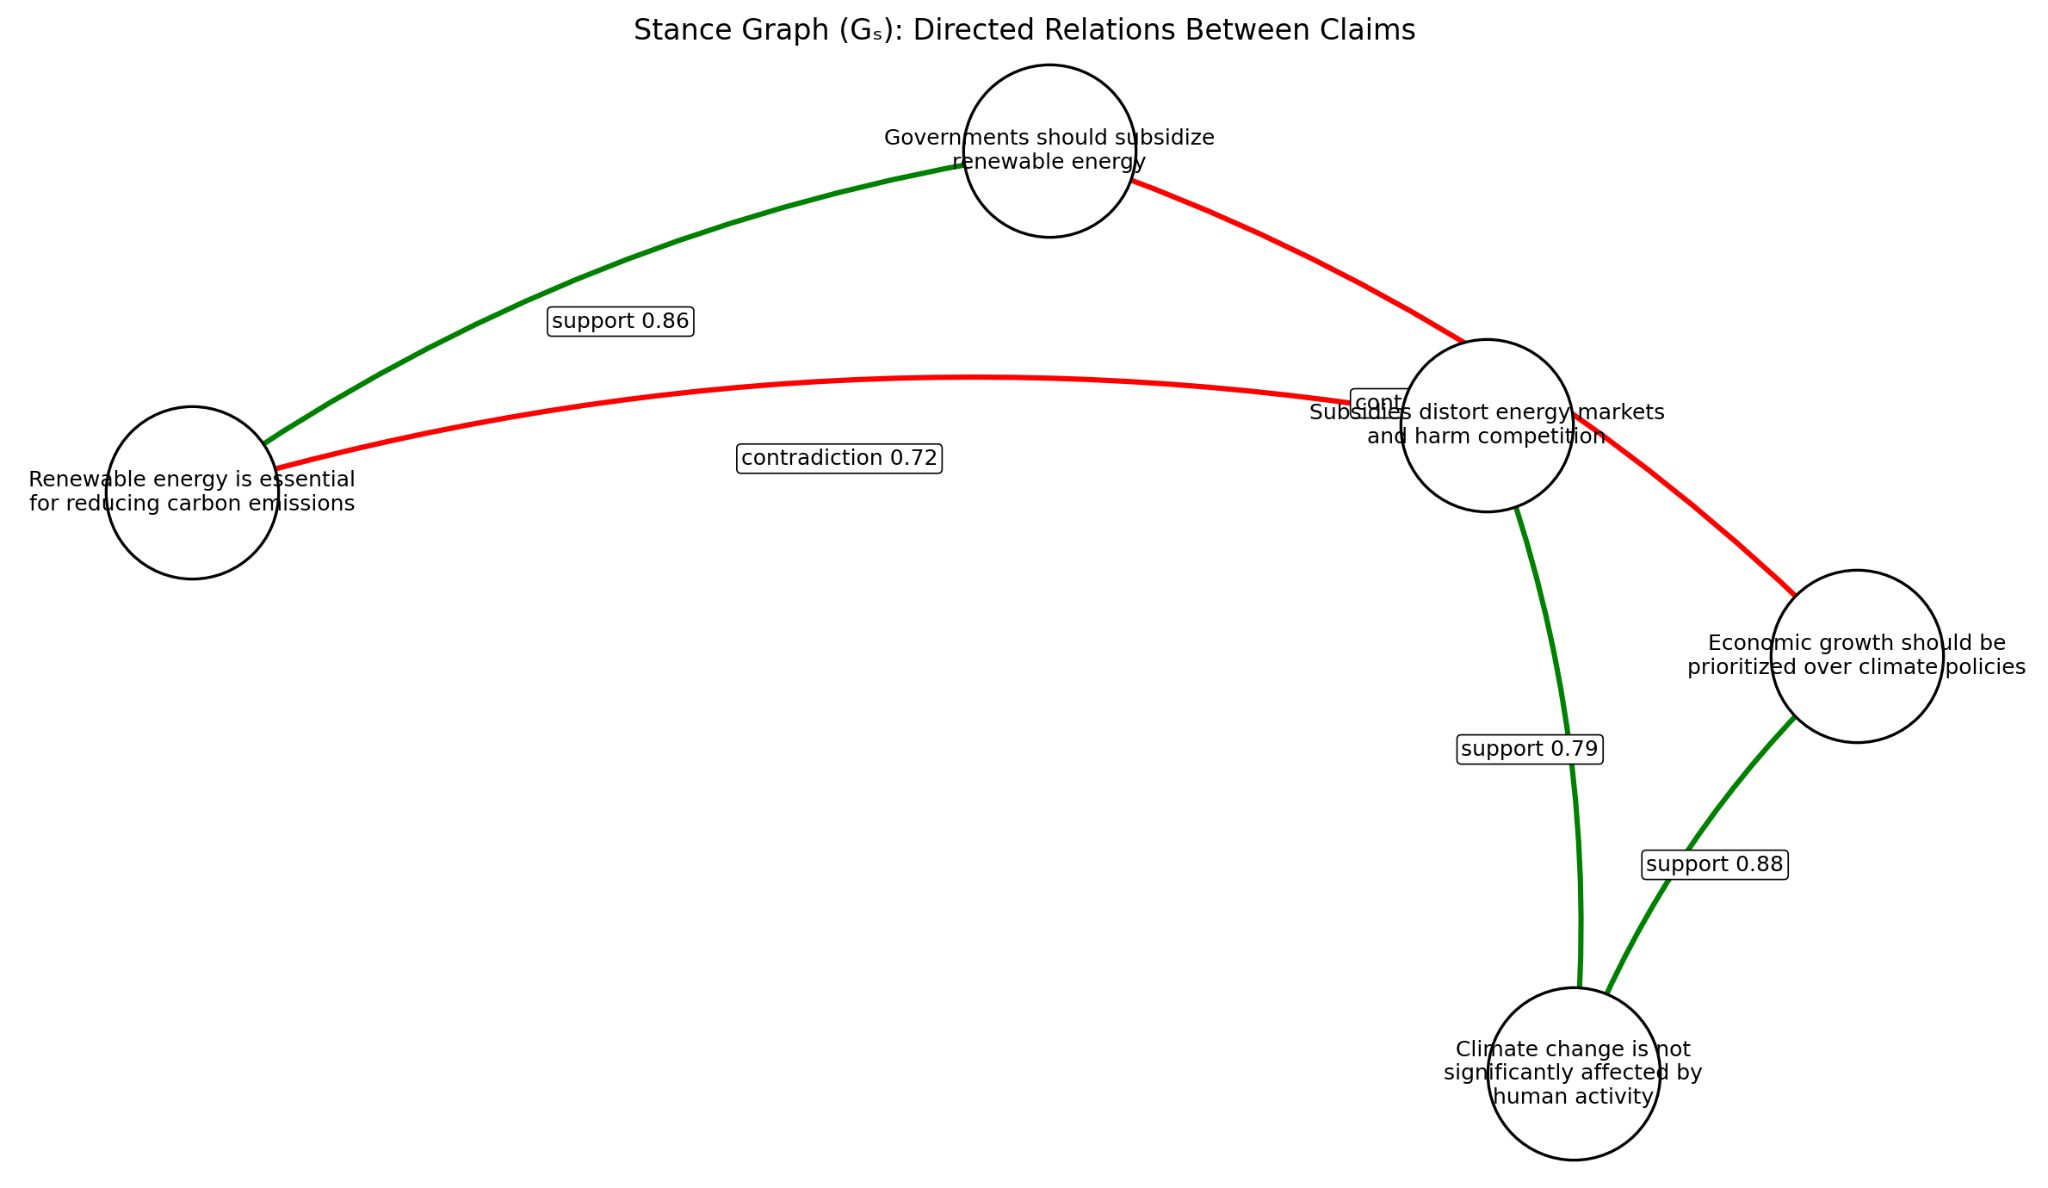
\includegraphics[width=0.86\linewidth]{2.png}
\end{frame}

\begin{frame}{Generated Logic Graph from Earlier Presentation}
\centering
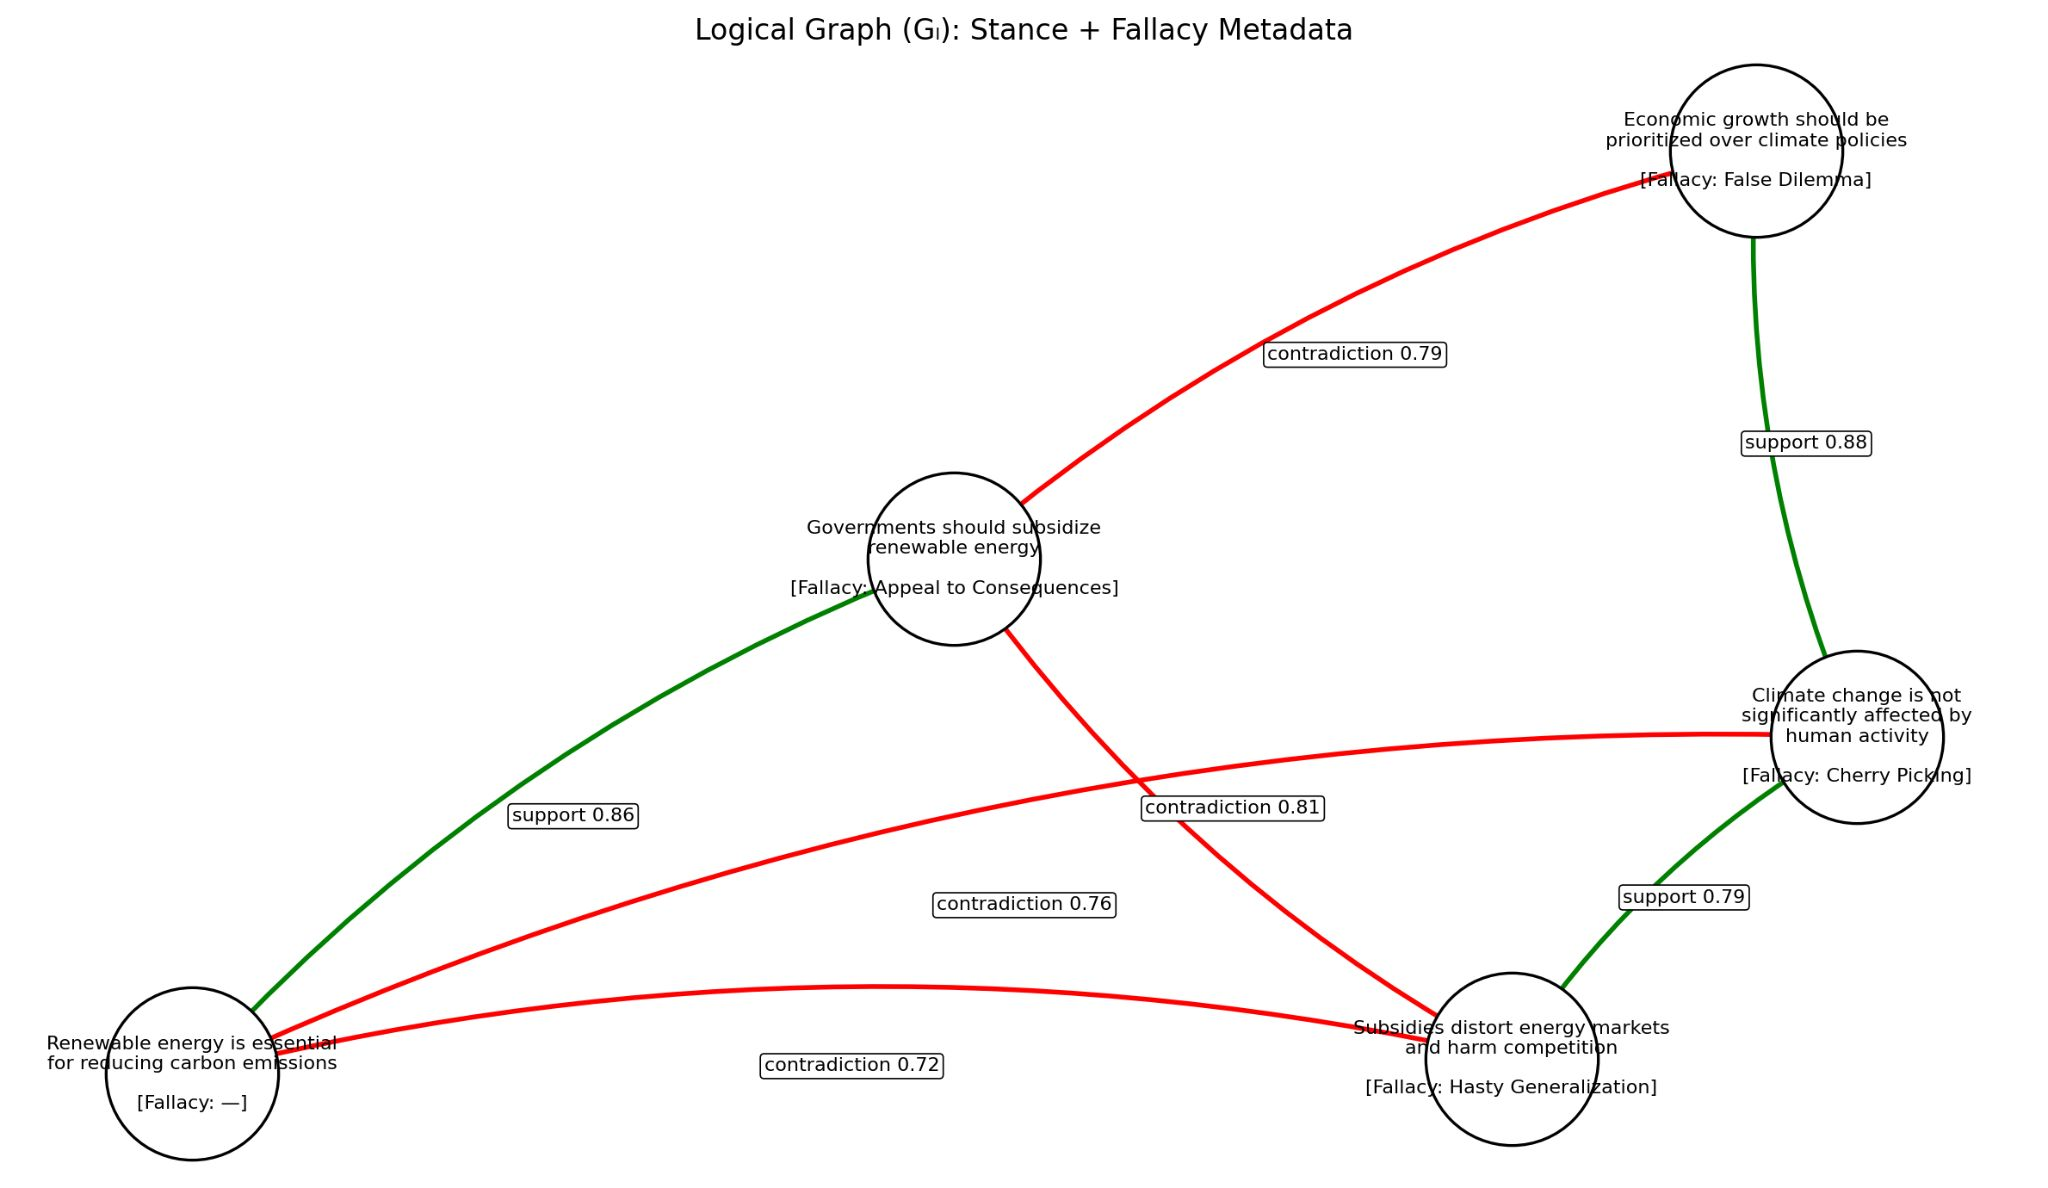
\includegraphics[width=0.86\linewidth]{3.png}
\end{frame}

\begin{frame}{Why Better Stance Detection Matters for Graph Analysis}
The earlier presentation already showed that downstream graph analysis depends on good edges:
\begin{itemize}
  \item Contradiction detection
  \item Cycle detection
  \item Support weakness analysis
  \item Clustering and discourse evolution
\end{itemize}

The graph-aware model improves these downstream stages because the graph itself becomes less noisy and more semantically coherent.
\end{frame}

\begin{frame}{Legacy Scalability Motivation}
  \begin{columns}[T]
    \begin{column}{0.52\textwidth}
      The earlier work also emphasized semantic pruning and scalability.

      This fits naturally with the graph-aware view:
      \begin{itemize}
        \item Not all claim pairs should be treated equally.
        \item Local semantic neighborhoods provide a principled way to restrict attention.
        \item Graph-aware stance prediction is therefore also a scalability-aware design direction.
      \end{itemize}
    \end{column}
    \begin{column}{0.43\textwidth}
      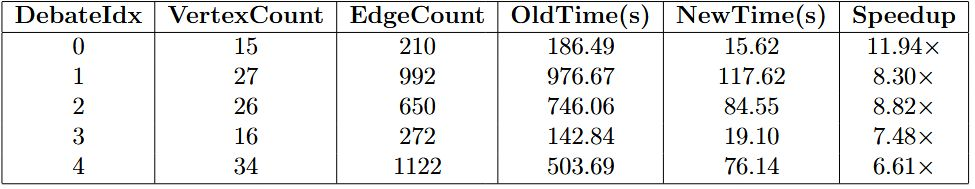
\includegraphics[width=\linewidth]{7.jpg}
    \end{column}
  \end{columns}
\end{frame}

\section{Conclusion}

\begin{frame}{Takeaways}
\begin{itemize}
  \item The main weakness of the old system was stance prediction, not graph reasoning itself.
  \item Direct NLI and direct stance baselines fail in opposite ways.
  \item DeBERTa + stance logistic regression is a strong non-graph baseline.
  \item The graph-aware model adds debate-local semantic structure and achieves the best results by a large margin.
\end{itemize}
\end{frame}

\begin{frame}{Next Research Steps}
\begin{itemize}
  \item Benchmark on more debates and multiple random seeds.
  \item Perform ablations over the 7 graph features.
  \item Compare TF--IDF graph features to embedding-based graph features.
  \item Move toward iterative graph refinement or a true graph neural model.
\end{itemize}
\end{frame}

\begin{frame}{Closing}
\centering
\Huge Thank You
\end{frame}

\end{document}
